\documentclass[a4paper,english]{book}

\usepackage[latin1]{inputenc}
\usepackage[T1]{fontenc}
\usepackage{fourier}
\usepackage{babel,textcomp}
\usepackage[pdftex]{graphicx}
\usepackage{subfigure}
\usepackage{listings}
\usepackage{hyperref}
\usepackage{varioref}
\usepackage{cite}
\usepackage[color]{uiosloforside}
\usepackage[bottom]{footmisc}
\usepackage{tikz}
\usetikzlibrary{shapes,arrows}
\usepackage[compact]{titlesec}
\usepackage{mdwlist}
\usepackage{multicol}
\usepackage{setspace}
\usepackage[subfigure]{tocloft}
\usepackage{fancyhdr}
\usepackage{chngcntr}
\counterwithout*{footnote}{chapter}
\setcounter{tocdepth}{1}

\setlength\topmargin{0in}
\setlength\topsep{0in}
\setlength\topskip{0in}
%\setlength\headheight{0in}
%\setlength\headsep{0in}
\setlength\textheight{9.0in}
\setlength\textwidth{6.5in}
\setlength\oddsidemargin{0in}
\setlength\evensidemargin{-0.25in}
\setlength\parindent{0in}
\setlength\parskip{0.10in}
\setlength\partopsep{0in}
\setlength\columnsep{0.25in}

\titlespacing{\section}{0pt}{*1}{*0}
\titlespacing{\subsection}{0pt}{*1}{*0}
\titlespacing{\subsubsection}{0pt}{*1}{*0}

\definecolor{dkgreen}{rgb}{0,0.6,0}
\definecolor{gray}{rgb}{0.5,0.5,0.5}
\definecolor{lightgray}{rgb}{0.8,0.8,0.8}
\definecolor{mauve}{rgb}{0.58,0,0.82}
\definecolor{matnat}{rgb}{0.004,0.47,0.44}

% Define Scala
\lstdefinelanguage{scala}{
  morekeywords={abstract,case,catch,class,def,
    do,else,extends,false,final,finally,
    for,if,implicit,import,match,mixin,
    new,null,object,override,package,
    private,protected,requires,return,sealed,
    super,this,throw,trait,true,try,
    type,val,var,while,with,yield},
  otherkeywords={=>,<-,<\%,<:,>:}, % Removed \#, @, because of Ruby comments error
  sensitive=true,
  morecomment=[l]{//},
  morecomment=[n]{/*}{*/},
  morestring=[b]",
  morestring=[b]',
  morestring=[b]"""
}

\lstset{basicstyle=\footnotesize,
  numbers=none,
  numberstyle=\tiny\color{gray},
  keywordstyle=\color{blue}\bfseries,
  commentstyle=\color{dkgreen},
  stringstyle=\color{mauve},
  frame=single,
  frameround=tttt,
  rulecolor=\color{lightgray},
  showstringspaces=false,
  breaklines=true,
  breakatwhitespace=true,
  tabsize=3,
  language=scala,
  captionpos=b,
  floatplacement=h,
}

\renewcommand{\lstlistlistingname}{List of Code Listings}

\hypersetup{pdfborder={0 0 0},colorlinks=false,linkcolor=blue,urlcolor=blue,citecolor=blue}

\newcommand{\matlab}{\textsc{Matlab}\textregistered}

\renewcommand{\headrulewidth}{0pt}
\fancyhead{}
\fancyfoot{}
\fancyhead[LE,RO]{\footnotesize \rightmark}
\fancyhead[LO,RE]{\footnotesize \leftmark}
\fancyfoot[LE,RO]{\thepage}
\fancypagestyle{plain}{
\fancyhead{}
\fancyfoot[LE,RO]{\thepage}}

\title{Embedding Efficient DSLs on the Java Virtual Machine}
\subtitle{A review of alternative languages}
\author{Eivind Barstad Waaler (\emph{eivindwa})}

\begin{document}
\uiosloforside[kind={Master thesis},boxcolor=matnat,textcolor=white]

{\pagestyle{plain}
\chapter*{Abstract}
\addcontentsline{toc}{chapter}{Abstract}

The Java Virtual Machine is an extremely popular software
platform\footnote{According to Sun there are over 4.5 billion
  JVM-enabled devices in the world --
  \url{http://www.java.com/en/about/}} capable of running programs in
the intermediate language called Java bytecode. The JVM supports a
wide range of languages\footnote{Wikipedia: List of JVM languages --
  \url{http://en.wikipedia.org/wiki/List_of_JVM_languages}} with
different typing, programming paradigm and compilation approach. This
thesis examines some of the most popular of these languages, with a
focus on embedding domain-specific languages. It is demonstrated how
various languages provide radically different possibilities, with
regard to syntax, composition, usage and performance. Examples are
given showing what programming languages are suited to particular
domain-specific tasks, and further research is suggested in the form
of new language features and new ways to utilize existing language
features.

\cleardoublepage
\addcontentsline{toc}{chapter}{Contents}
%\begin{multicols}{2}
\tableofcontents
%\end{multicols}

\clearpage
\addcontentsline{toc}{chapter}{List of Tables}
\listoftables

\addcontentsline{toc}{chapter}{List of Figures}
\listoffigures

\clearpage
\begin{multicols}{2}
\addcontentsline{toc}{chapter}{List of Code Listings}
\lstlistoflistings
\end{multicols}

\chapter*{Preface}
\addcontentsline{toc}{chapter}{Preface}

This is a master-thesis of 60 credits\footnote{Prescribed to one year
  of full time study.} in the field of Informatics. It was written for
the Object-orientation, Modelling, and Languages research
group\footnote{OMS research group website --
  \url{http://www.ifi.uio.no/research/groups/oms/}} at the Department
of Informatics, Faculty of Mathematics and Natural Sciences,
University of Oslo.

I want to thank my wonderful wife Anniken for the support and
understanding she has shown during this process.

My thanks and thoughts also go to the memory of my grandfather Bjarne
A. Waaler. His constant search for knowledge and truth has been an
enormous inspiration all my life. I am proud to make a contribution to
the same university where he spent so many of his years working, both
in research and administration.

At last, but not least, I would like to thank my supervisor Professor
Birger M�ller-Pedersen at the Department of Informatics, UiO. His
unique experience from projects such as the \textsc{beta} programming
language and the \textsc{swat} project has proven extremely valuable
for me. Through many good discussions at his office I've learned much
about current and historic programming language concepts. His
enthusiasm has motivated me from beginning to end.

\begin{flushright}
\textsc{Eivind Barstad Waaler}\\
Oslo, Norway\\
May 2010
\end{flushright}

\chapter{Introduction}
\label{chp:introduction}
}\pagestyle{fancy}

The goal of this chapter is to describe the problem at hand as
detailed as possible. It has taken me a long time to clarify and
understand the problem, and as such I think it is justified to spend
quite a lot of time and space describing the background and why it is
important. First the problem formulation is given, with a brief
background and motivational description. The rest of the chapter
describes the method followed, and gives more detailed explanations of
the terminology and background of choices made regarding the problem
formulation. The final section gives a brief outline of how the rest
of the report is structured.

\section{Problem Description}
\label{sec:problemdescription}

\subsection{Problem Formulation}
\label{sec:problemformulation}

\textit{Evaluate some major alternative programming languages on the
  Java Virtual Machine with regards to embedding domain-specific
  languages. Identify important aspects when working with embedded
  domain-specific languages and show what programming languages are
  suited and how they solve the problems.}

\subsection{Background}
\label{sec:background}

A domain-specific language (DSL\footnote{Also known as
  problem-oriented or special-purpose programming language in computer
  literature.}) is a programming language dedicated to a particular
problem domain. This thesis looks at embedding such DSLs into existing
general-purpose programming languages, with a focus on several
categories of languages with different features, and how these
features are used. The scope is limited to the platform offered by the
Java Virtual Machine, and a set of programming languages (described
further in chapter \vref{chp:examples}). A more detailed definition of
domain-specific languages, with a discussion around scoping and
requirements, is given in section \vref{sec:dsls}.

\subsection{Motivation}
\label{sec:motivation}

I have 10 years experience using the Java programming language,
working as a professional consultant for BEKK\footnote{Bekk Consulting
  AS (\url{http://www.bekk.no}).}. I have always been fascinated by
various programming languages, and how they can be used to approach
problems and solutions. When starting on a master thesis it is natural
for me to focus on programming language capabilities. I feel that the
embedded DSL domain provides a good basis for exploring different
categories of programming languages, and by limiting the focus to the
Java Virtual Machine I can control the scope and draw on my experience
working with the Java platform.

\section{Method}
\label{sec:method}

This section describes the research method applied in the
thesis. In\cite{dyb08} the concept ``Evidence-Based Software
Engineering'' (EBSE) is introduced. It describes a method that can be
used when making decisions in Software Engineering, combining evidence
found in literature with practical experience and conducted
experiments. Although the method is mainly targeted towards
practitioners looking to support decision-making it can easily be
adapted to support an evaluative thesis as this one. The main steps of
EBSE are as follows:

\begin{enumerate*}
\item Convert a relevant problem or need for information into an
  answerable question.
\item Search the literature for the best available evidence to answer
  the question.
\item Critically appraise the evidence for its validity, impact, and
  applicability.
\item Integrate the appraised evidence with practical experience and
  the client's values and circumstances to make decisions about
  practice.
\item Evaluate performance in comparison with previous performance and
  seek ways to improve it.
\end{enumerate*}

With this list as basis I have built a list of steps that I will
follow in the thesis work. To summarize I will use existing literature
extensively to build a solid base for the experiments conducted, and
try to critically conclude the work at the end:

\begin{enumerate*}
\item Identify requirement -- Make sure the questions to research are
  sound and possible to answer.
\item Search theory -- Find literature to provide direct answers to
  the questions, or to support assumptions needed to sustain
  experiments.
\item Write example -- The major part of the thesis work is of course
  related to the experiments conducted. The first two steps are
  important to make sure the experiments are based on sound evidence
  and former knowledge.
\item Measure -- Measure results, if applicable. Those results that
  produce some kind of measurable unit will be included in this phase.
\item Conclude -- Make a preliminary conclusion based on the results
  found so far.
\item Evaluate -- The experiments and results found must be carefully
  evaluated. By being critical to my own results I hope to improve the
  overall quality of the thesis deliverance.
\end{enumerate*}

The process is illustrated in figure \vref{fig:method}. Not all the
phases are relevant for all requirements investigated. As shown with
the dotted lines, a conclusion might be deducted directly from theory,
and the measurement phase is not necessarily valid for all
requirements. Note also that the method is used iteratively, in
cycles, after evaluation of the results new or modified requirements
can be taken into consideration. This way of working is very good for
a master thesis of a set time/size, as the method is simply run over
and over again as many times as there is room for.

\begin{figure}[h]
  \begin{center}
  \tikzstyle{line} = [draw, -latex']
  \tikzstyle{cloud} = [rectangle, draw, text width=6em, text centered, rounded corners, node distance=3.5cm, minimum height=5em]
  %\tikzstyle{cloud} = [draw, ellipse,fill=red!20, text width=5em, text centered, node distance=4.5cm, minimum height=5em]
  \begin{tikzpicture}[node distance = 2cm, auto]
    % Place nodes
    \node [cloud, fill=blue!5] (requirement) {1. Identify requirement};
    \node [cloud, fill=blue!10, right of=requirement, above of=requirement] (theory) {2. Search theory};
    \node [cloud, fill=blue!30, right of=requirement, below of=requirement] (evaluate) {6. Evaluate};
    \node [cloud, fill=blue!15, right of=theory] (example) {3. Write example};
    \node [cloud, fill=blue!25, right of=evaluate] (conclude) {5. Conclude};
    \node [cloud, fill=blue!20, right of=example, below of=example] (measure) {4. Measure};
    % Draw edges
    \path [line] (requirement) -- (theory);
    \path [line] (theory) -- (example);
    \path [line] (example) -- (measure);
    \path [line] (measure) -- (conclude);
    \path [line] (conclude) -- (evaluate);
    \path [line] (evaluate) -- (requirement);
    \path [line, dotted] (theory) -- (conclude);
    \path [line, dotted] (example) -- (conclude);
  \end{tikzpicture}
  \end{center}
  \caption{Illustration of method phases.\label{fig:method}}
\end{figure}

\subsubsection{A Note on Theory/Literature}

Many of the programming languages used in this thesis are relatively
new, and not commonly studied in much academic research yet. Much of
the most recent material written on or about the languages exist in
less formal ways, typically as Internet articles or blog posts. I have
tried to use scientific research papers as theory basis as much as
possible, but a certain amount of references/footnotes will also refer
to links on the Internet. Although not as reliable as scientific
resources, I find it more honest to include the source of any
ideas/inspiration.

\section{Domain-Specific Languages}
\label{sec:dsls}

\textit{``Domain-specific languages (DSLs) are languages tailored to a
  specific application domain. They offer substantial gains in
  expressiveness and ease of use compared with general-purpose
  programming languages.''}\cite{mer05}

DSLs are often categorized in two major types; external or embedded
(also referred to as internal) DSLs. An external DSL is a separate
programming language with custom syntax and a full parser. Some
well-known examples of external DSLs are SQL (domain of database
queries), CSS (domain of HTML styles) and XML (domain of data
exchange). An embedded DSL on the other hand, is created in a host
language. Various capabilities in the host language are exploited to
create interfaces that look and behave almost like a particular
programming language.

In this thesis I have identified different requirements of embedded
DSLs running on the Java Virtual Machine (JVM), and looked at how
various programming languages (described in section
\vref{sec:programminglanguages}) solve these aspects. As described in
the next section the exact definition of an embedded DSL is hard to
find, and as such this thesis is just as much a study of different
programming languages and what capabilities they provide. The embedded
DSL focus provides examples used to visualize and compare results.

\subsection{Embedded DSL or just Advanced Library Design?}
\label{sec:embeddeddsl}

It is difficult to draw a precise line between an embedded DSL and a
regular library. If you have a library specialized to solve problems
in a given domain, is that enough to call it an embedded DSL? How much
``special syntax'' do you need to include in the library to make it a
DSL? What kind of syntax qualifies for DSL use? Answering questions
like these is difficult, and in my opinion not contributing to a
fruitful discussion. I have tried to turn my focus toward interesting
capabilities different languages have, and the problems they solve. As
such some of the examples I will be using might not qualify as
embedded DSLs, but merely as libraries/interfaces with nontraditional,
or in other ways interesting, use of the host language.

Martin Fowler and Eric Evans have defined the name ``fluent
interface''\cite{fow05} to describe interfaces which provide a more
readable and ``flowing'' syntax. Many of the examples given of fluent
interfaces are small libraries solving tasks in a specific domain, and
as such are also good examples of embedded DSLs. Eric Evans has also
written a book\cite{eva04} and held a number of talks on the subject
of Domain-Driven Design (DDD), a way of thinking and prioritizing when
working with software projects that deal with complicated domains. DDD
hardly covers the subject of embedding DSLs, but I feel that a lot of
the DSL design is focused on understanding and expressing a particular
domain and as such has a lot in common with the thoughts behind DDD.

The reason this discussion was included is to briefly try to
demonstrate that the area of embedded DSLs is a complex and maybe not
precisely defined one. The activity of building an embedded DSL is
tightly connected to the understanding of the domain at hand, and the
capabilities required from the host language will vary strongly with
that understanding. The next section gives a list of such
requirements.

\subsection{Requirements of an Embedded DSL}
\label{sec:requirements}

The following lists the different requirements/capabilities that I
have considered in this work. The list provides a foundation for
structuring the rest of this report:

\begin{itemize}
\item \textbf{Syntax Conciseness/``fluency''} -- What capabilities
  does the different languages provide in building fluent interfaces?
\item \textbf{Modularity/composition} -- How can several DSLs be
  combined/reused into new ones?
\item \textbf{Isolation/uniqueness} -- How can unwanted features of
  the host language be deprecated/removed? How can the host language
  be extended to provide new functionality?
\item \textbf{Use} -- How can embedded DSLs be used? What is the level
  of tool support provided for the DSL? How are errors and exceptional
  situations handled in the different languages?
\item \textbf{Performance} -- How does the different languages
  facilitate building DSLs with high demands regarding
  throughput/performance?
\end{itemize}

\section{Report Structure}

The rest of this report is structured around the requirements listed
in section \ref{sec:requirements}. After a brief description of the
programming languages used, and the examples studied, each of the
requirements are treated in separate chapters. As described in the
method section, each requirement is studied in terms of existing
literature combined with examples. A summary is written for each
chapter, concluding the results found related to the requirements
covered by the chapter.

Chapter \ref{chp:examples} <<Programming Languages and Examples>>
describes the programming languages used and the example DSLs created
or studied in this thesis.  Chapter \ref{chp:syntax} <<Syntax>> looks
at techniques for creating concise and ``fluent'' syntax.  Chapter
\ref{chp:composition} <<Composition>> handles composition of DSLs.
Chapter \ref{chp:advancedtechniques} <<Advanced Techniques>> describes
advanced DSL techniques like pruning (removing features from) and
extending the host language.  Chapter \ref{chp:dsluse} <<Exploring
Ways to Use Embedded DSLs>> handles different ways to utilize and run
the DSLs.  Chapter \ref{chp:performance} <<Performance>> discusses
various aspects regarding DSL performance.  Chapter \ref{chp:summary}
<<Summary>> provides a summary containing the conclusion as well as
some suggestions to further work.

\clearpage{\pagestyle{plain}\cleardoublepage}

\chapter{Programming Languages and Examples}
\label{chp:examples}

This chapter introduces the programming languages used in the thesis,
and the DSL examples studied. As described in the introduction the
main focus has been on capabilities provided by a set of different
programming languages, and how these capabilities sustain the
development of various types of embedded domain-specific
languages. Some examples have been developed as part of the work,
while other examples have been taken from existing frameworks.

\section{JVM Programming Languages}
\label{sec:programminglanguages}

The goal platform of this thesis is the Java Virtual Machine
(JVM). The reason for this is that the enormous popularity of the Java
programming language has made the JVM one of the most widespread
multi-language platforms in the world. At the same time the Java
language itself is getting old, and many other languages have been
written (or ported) for the JVM. So this thesis looks at how some of
these languages provide various capabilities when building embedded
DSLs. I have tried to look at languages that differ in many
categories, as typing, paradigm or execution model. The languages
studied are described and categorized in the next sections.

\subsection{Categories of Languages}

I have chosen to categorize the languages in three different ways:

\begin{itemize}
\item \textbf{Typing (static/dynamic)} -- Static typing means that the
  majority of the type checking of the language is enforced during
  compile-time, as opposed to run-time. The opposite is dynamic typing
  which performs most of the type checking during run-time.
\item \textbf{Paradigm (OO/FP)} -- There are many different
  programming paradigms. I have looked at object-oriented and
  functional programming languages. Some of the languages (Ruby,
  Groovy and Scala) are multi-paradigm languages, combining
  object-orientation and functional programming techniques.
\item \textbf{Execution (compiled/interpreted)} -- On the JVM an
  interesting way to categorize programming languages is whether they
  are compiled to byte-code and run directly on the virtual machine,
  or if the language is interpreted and run by some extra layer on top
  of the JVM.
\end{itemize}

Table \vref{tab:plmatrix} shows the languages used in the thesis, and
what categories they belong to. An \texttt{(x)} denotes partial
support, a non-default configuration possibility, or that the language
supports something similar. For example are both Groovy and Ruby said
to support some notion of functional programming, although it is not
their main focus. Scala and Clojure are both compiled languages that
can be run in a REPL, a Read-Eval-Print-Loop compiling statements on
the fly making it seem like they are interpreted. This gives both
languages the possibility to run as scripts or directly in the
console, as if they were interpreted (not compiled) languages.

\begin{table}[ht]
  \centering
  \begin{tabular*}{1\textwidth}{l c c c c c c}
    \hline
    & Object-oriented & Functional & Static Typing & Dynamic Typing & Compiled & Interpreted \\ [0.5ex]
    \hline
    Java & x & - & x & - & x & - \\
    Groovy & x & (x) & - & x & (x) & x \\
    Ruby & x & (x) & - & x & (x) & x \\
    Clojure & - & x & - & x & x & (x) \\
    Scala & x & x & x & - & x & (x) \\
    \hline
  \end{tabular*}
  \caption{Programming languages comparison matrix.\label{tab:plmatrix}}
\end{table}

Each of the languages are further introduced in the following
sections.

\subsection{Java}

Java is naturally the most common programming language used on the
JVM. It is a statically typed and compiled language supporting the
object-oriented paradigm. It provides the baseline for the work, and
will be used as example language where applicable. Much of the work
however has gone in showing how other languages provide features
useful when building DSLs, features not currently found in the Java
language itself. So Java will also be used quite heavily for reference
and comparison to the other languages. It is assumed that the reader
has a certain knowledge about the Java language (because of its wide
adoption in both academic and enterprise environments), and many Java
concepts will only be described briefly or referred to without
explanaition.

Embedded DSLs can also be written in Java. A good background with
examples can be found in\cite{fre06}, a paper describing the
development of the testing framework \texttt{jMock} as an embedded DSL
in Java. The techniques described in\cite{fre06} can be seen as a sort
of baseline for what is possible in Java. The majority of work done in
this report is showing what can be achieved using features from other
languages, going beyond what is capable in the Java language. The
example shown in listing \vref{lst:jmock} is from\cite{fre06}, showing
the DSL syntax of mock object expectations used in a mock
\texttt{Offer} class.

\begin{lstlisting}[float,caption=Java jMock example.,label=lst:jmock,language=java]
void testAcceptsOfferIfLowPrice() {
  offer = mock(Offer.class);
  offer.expects( once() )
       .method( "buy" )
       .with( eq(QUANTITY) )
       .will( returnValue(receipt) );
  ...
}
\end{lstlisting}

\subsection{Groovy}

Groovy is a dynamically typed and compiled language supporting the
object-oriented paradigm. It is tightly integrated with Java and can
leverage existing Java libraries directly. An example of a simple
object-oriented ``Hello World!'' program is shown in the following
example:

\begin{lstlisting}[language=java,caption=Groovy ``hello world'' example.,label=lst:groovyhello]
class Greet {
  def name

  Greet(who) { name = who }

  def salute() { println "Hello \$name!" }
}

// Groovy comments are the same as in Java
new Greet('world').salute()
\end{lstlisting}

I have included Groovy in this thesis as it provides an interesting
dynamically typed alternative to the Java language. It has some
syntax-capabilities making it well suited for building embedded DSLs.

\subsubsection{Groovy and Java}

Groovy is very tightly integrated with Java. In most cases, an
existing Java code file can be renamed to \texttt{.groovy} and run
directly. This is due to the fact that Groovy supports most of the
native Java syntax, as well as all the ``new'' dynamic style
syntax. All Java classes can be imported and used directly in Groovy.

\subsection{Ruby/JRuby}

Ruby is a dynamically typed and interpreted language supporting the
object-oriented paradigm. JRuby is a Java implementation of the Ruby
language on the JVM, thus acting as an interpreter for Ruby on the
JVM. The latest versions of JRuby also support some notions of
just-in-time compilation, as well as regular ahead-of-time
compilation.

The main reason for my inclusion of Ruby in this thesis is the ``Ruby
on Rails'' framework\cite{rails}, an extraordinary DSL running on the
JVM with the help of the JRuby interpreter. In listing
\vref{lst:rubyhello} is a Ruby implementation of the same ``hello
world'' program that was shown in Groovy in the previous section.

\begin{lstlisting}[float,caption=Ruby ``hello world'' example.,label=lst:rubyhello,language=ruby]
class Greet
  @name

  def initialize(name)
    @name = name
  end

  def salute()
    puts "Hello #@name!"
  end
end

# A Ruby comment
Greet.new("world").salute()
\end{lstlisting}

\subsubsection{JRuby and Java}

JRuby can use classes from the standard Java API directly using the
\texttt{include Java} statement. It can also import Java classes
directly from jar files. So most Java libraries and APIs can be reused
when working with JRuby on the JVM. An example of this is shown in
listing \vref{lst:rubyjava} (creating a Java Swing application).

\begin{lstlisting}[float,caption=Ruby Java integration example.,label=lst:rubyjava,language=ruby]
# Special include to make standard Java API available
include Java

frame = javax.swing.JFrame.new("Main Window")
frame.getContentPane.add(javax.swing.JLabel("Press button:"))
frame.getContentPane.add(javax.swing.JButton("OK"))
frame.setDefaultCloseOperation(javax.swing.JFrame::EXIT_ON_CLOSE)
frame.pack
frame.setVisible(true)
\end{lstlisting}

\subsection{Clojure}

Clojure is a dynamically typed and compiled language supporting the
functional programming paradigm. It is a modern dialect of the LISP
programming language compiling to Java bytecode. It is the only
language not supporting object-orientation directly, and also the
youngest and possibly the least mature language included in my work.

The reason I have looked at Clojure is the amount of embedded DSL
papers written using functional programming languages (for
example\cite{hud96}), making Clojure an interesting language with
respect to embedding DSLs on the JVM. Below is an example of the
``hello world'' function in Clojure, as well as an example
implementation of the Fibonacci function (a more common ``hello
world'' in the functional world):

\begin{lstlisting}[language=lisp,caption=Clojure Fibonacci example.,label=lst:clojurefibonacci]
; A kind of hello world function
(def hello (fn [] "Hello world"))

; The fibonacci function
(defn fib [n] 
  (if (<= n 1) 
    1
    (+ (fib (- n 1)) (fib (- n 2)))
  )
)
\end{lstlisting}

\subsubsection{Clojure and Java}

Clojure is the language studied that has the least in common with
Java, with regards to syntax and appearance. Many people not being
used to the syntax of LISP might find Clojure difficult to read, with
all the parenthesis being a central part of the structure. Figure
\vref{fig:cljjava} shows a basic example with a variable, function and
some output, implemented side by side in Clojure and Java. In many
ways Clojure is much more consistent in its syntax. While Java has
special keywords and forms for defining variables, functions, operator
use and more, Clojure simply does everything the same way. Notice how
the definition of the variable in Clojure is the same as the
definition of the function, and that the comparison operator used in
the if statement in Java is also just a regular function in the same
form as the definitions in Clojure. Once you get used to the Clojure
way, Java might not feel so consistent anymore.

\begin{figure}[t]
  \subfigure[Clojure]{\lstinputlisting[nolol,language=lisp,linewidth=0.48\textwidth]{../examples/clj-java/ex.clj}}
  \hspace{37pt}
  \subfigure[Java]{\lstinputlisting[nolol,language=java,linewidth=0.48\textwidth]{../examples/clj-java/ex.java}}
  \caption{Example comparing syntax consistency of Clojure and Java side by side.\label{fig:cljjava}}
\end{figure}

Clojure integrates with Java using some special macros like
\texttt{import} and \texttt{new}, and the dot operator, as shown in
the examples given in listing \vref{lst:clojurejava}.

\begin{lstlisting}[float,caption=Clojure -- Java integration.,label=lst:clojurejava,language=lisp]
; Get a system property
(System/getProperty "java.vm.version")
; Call "toUpperCase" on the String "clojure"
(.toUpperCase "clojure")
; Import java.util.Date, make a new instance and print the class name
(import java.util.Date)
(new Date) ; New instance of Date
(.getName Date) ; Call "getName" on the Date class
\end{lstlisting}

In addition all Clojure data structures implement standard Java
interfaces, making it easy to run code implemented in Clojure from
Java. The very good interoperability between Clojure and Java is a bit
surprising looking at the extreme differences in syntax and
programming paradigm, but is a powerful addition to the LISP
world. Combining the macros of a LISP language with all the available
libraries on the Java platform seems to be a very good idea. A good
book for learning more about Clojure is <<Programming
Clojure>>\cite{hal09}.

\subsection{Scala}

\textit{``Scala is a general purpose programming language designed to
  express common programming patterns in a concise, elegant, and
  type-safe way. It smoothly integrates features of object-oriented
  and functional languages, enabling Java and other programmers to be
  more productive. Code sizes are typically reduced by a factor of two
  to three when compared to an equivalent Java
  application''.}\cite{scala}

Scala is a relatively new language (first version released
2003\cite{scala}) providing exciting programming capabilities on the
Java Virtual Machine (JVM). The main reason for choosing Scala in this
thesis is the combination of powerful programming structures (both
object-oriented and functional) with the cross-platform and wide
adoption of the JVM. Code written in Scala can be run on any JVM
version 1.5 or newer, and can utilize any library written in Java. It
can thus be seen as a ``best of both worlds'' language.

For more detailed information about Scala please refer
to\cite{ode08},\cite{scala} or\cite{scalatour}.

\subsubsection{Scala and Java}
\label{sec:scalajava}

Scala code (.scala files) compiles to Java bytecode (.class files)
through a special compiler (\texttt{scalac}). The bytecode can then be
run on the JVM as if it was created from Java source (.java files). In
addition Scala provides a number of library classes that need to be
included as a jar file. This relationship between Scala and Java is
illustrated in figure \vref{fig:scalajava}.

\begin{figure}[h]
  \begin{center}
  \tikzstyle{block} = [rectangle, draw, fill=blue!20, text width=5em, text centered, rounded corners, minimum height=4em]
  \tikzstyle{line} = [draw, -latex']
  \tikzstyle{cloud} = [draw, ellipse,fill=red!20, text width=5em, text centered, node distance=2.5cm, minimum height=2em]
  \begin{tikzpicture}[node distance = 2cm, auto]
    % Place nodes
    \node [cloud] (class) {Java Bytecode (.class)};
    \node [block, left of=class, above of=class] (scalacompile) {Scala Compile (scalac)};
    \node [cloud, left of=scalacompile] (scala) {Scala Source (.scala)};
    \node [block, right of=class, above of=class] (javacompile) {Java Compile (javac)};
    \node [cloud, right of=javacompile] (java) {Java Source (.java)};
    \node [block, below of=class] (jvm) {Java Virtual Machine};
    \node [block, below of=scala] (scalalib) {Scala API (.jar)};
    % Draw edges
    \path [line] (scalacompile) -- (class);
    \path [line] (javacompile) -- (class);
    \path [line] (class) -- (jvm);
    \path [line] (scala) -- (scalacompile);
    \path [line] (java) -- (javacompile);
    \path [dotted, line] (scalalib) -- (jvm);
  \end{tikzpicture}
  \end{center}
  \caption{Visual representation of the relationship between Scala and
    Java.\label{fig:scalajava}}
\end{figure}

The tight relationship with Java has a number of advantages when using
Scala:

\begin{itemize}
\item Cross-platform distribution -- Code written in Scala can be run
  on any platform supporting JVM 1.5 or newer.
\item Stability and standards -- The JVM is a stable platform with
  good support for internationalization (Unicode support ++) and
  localization (supports local languages and standards).
\item Access to libraries -- The JVM has a wide range of libraries
  available, many being Open Source.
\item High performance -- The JVM has been proven to be a high
  performance Virtual Machine, with a large number of tuning
  possibilities.
\end{itemize}

There are also disadvantages with such a tight coupling to the JVM:

\begin{itemize}
\item Limitations in bytecode -- Scala, being a functional language,
  would benefit from features not present in the current version of
  the JVM. Most notably is the (lack of) support for full tail call
  optimization, which would improve performance of recursive
  functions.
\item Generics implemented with erasure -- Scala uses an erasure
  scheme to implement generics, to be 100\% compatible with
  Java. However, the implementation of the Scala compiler
  (\texttt{scalac}) has some advanced solution to many of the problems
  Java has regarding erasure\cite{emi06}.
\end{itemize}

\section{Examples Implemented}

This section describes the main examples written and researched in the
thesis. The DSLs are described, and details about implementation and
key features given. Some source code being central in the
implementation is shown in the text. Full source code for all the
examples can be downloaded from my repositories at
GitHub\footnote{GitHub repositories website --
  \url{http://github.com/eivindw}}.

\subsection{DSL for Image Processing}
\label{sec:dslimageprocessing}

\subsubsection{Description}

Image Processing is an area involving series of computationally heavy
operations performed on images\cite{gon08}. Many practitioners in the
area have more mathematical than computer science oriented
background. This leads to the need for DSLs where complicated and
computationally heavy operations can be performed with a simple and
straightforward syntax.

A major actor in the art of Image Processing is the product \matlab{}
from the company MathWorks\texttrademark. They provide the user with a
DSL for doing advanced Image Processing operations. The goal of this
example is to create a similar DSL (with a limited amount of
functionality) running on a JVM. This DSL was implemented in Scala,
mostly due to performance requirements.

As an example consider the operation of blurring an image using an
average filter mask show in figures \vref{fig:eximg} and
\vref{fig:exavg}. This is a basic operation, documented
in\cite{gon08}, but serves good as an example of using the DSLs.

The \matlab{} code to perform the operation could
typically look like this:

\begin{lstlisting}[language=matlab,caption=\matlab{} image processing example.,label=lst:matlabimgproc]
img = imread('cell.jpg');
% 3x3 neighborhood default
imgAvg = medfilt2(img);
imwrite(imgAvg, 'cell_avg.jpg');
\end{lstlisting}

A Scala-solution to the same problem is shown in listing
\vref{lst:scalaimgproc}. The rest of this section describes how this
was implemented, with regards to syntax and class/object
composition. The DSL also implements basic morphological operations
like erode, dilate, open and close\cite{gon08}.

\begin{lstlisting}[float,caption=Scala image processing example.,label=lst:scalaimgproc]
// Imports...
val img = loadImageCP("/cell.jpg")
val se = StrEl(Square, 3)
val imgAvg = img.avg(se)
saveImage(imgAvg, "/cell_avg.jpg")
\end{lstlisting}

TODO: Replace image with something I have taken myself.

\begin{figure}
  \subfigure[Original]{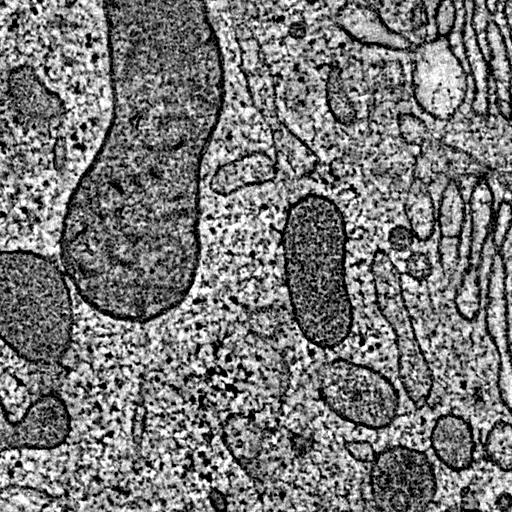
\includegraphics[width=0.49\textwidth]{images/cell}}
  \hfill
  \subfigure[Blurred]{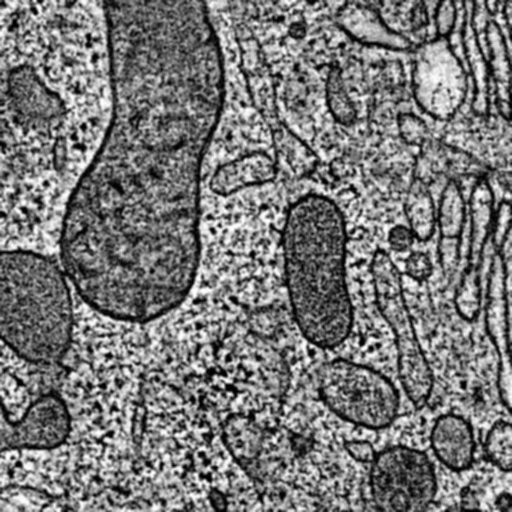
\includegraphics[width=0.49\textwidth]{images/cell_avg}}
  \caption{Example image before and after blurring with average
    filter.\label{fig:eximg}}
\end{figure}

\begin{figure}
  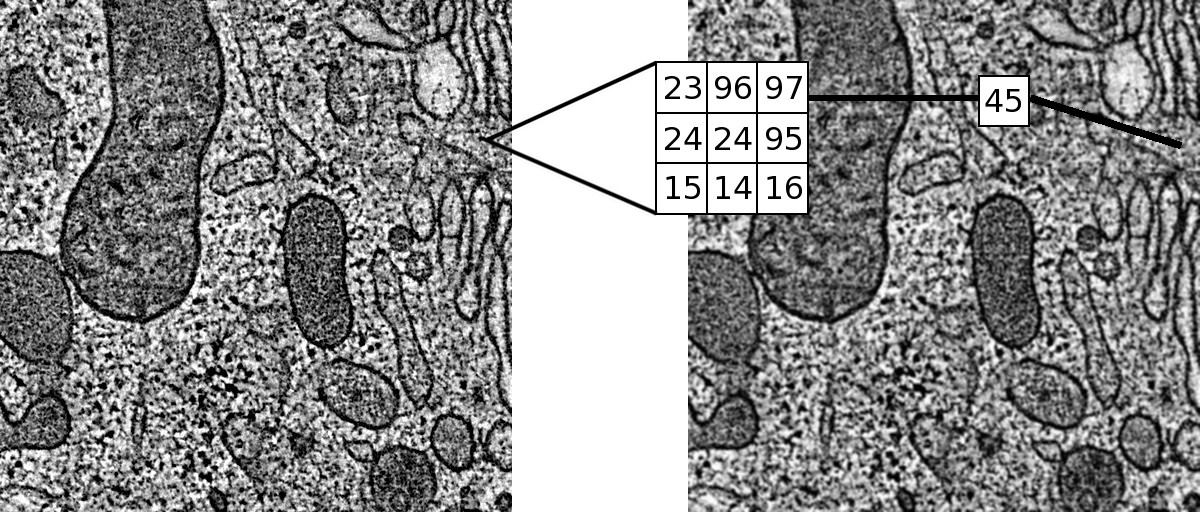
\includegraphics[width=1.0\textwidth]{images/avg_process}
  \caption{Visualising the process of blurring an image using average
    filtering with a 3x3 neighbourhood.\label{fig:exavg}}
\end{figure}

\subsubsection{Syntax}

This section briefly describes the syntax and implementation of the
example. Some Scala features are used that will be further explained
in the next chapter, and are only described here with short footnotes.

The methods to load and save the image, as well as the \texttt{Square}
definition of structuring element, are all member functions in classes
\texttt{SImageIO} and \texttt{StrElType}. These can be imported with
the \texttt{.\_} notation in Scala, and are then available
directly\footnote{The Scala member import is similar to the static
  member import found in Java, making static methods in a class
  directly available.}. An example is shown in listing
\vref{lst:scalaipsyn}, where the comments show how the statements
would look without using the static member import.

\begin{lstlisting}[caption=Scala image processing syntax example.,label=lst:scalaipsyn]
import io.SImageIO._
import structs.StrElType._

// SImageIO.loadImageCP("/cell.jpg")
val img = loadImageCP("/cell.jpg")
...
saveImage(imgAvg, "/cell_avg.jpg")

// StrElType.Square
val se = StrEl(Square, 3)
\end{lstlisting}

To create the structuring element, the \texttt{StrEl} trait has a
``companion object''\footnote{A companion object is a singleton
  \texttt{object} having the same name as an associated \texttt{trait}
  or \texttt{class}\cite{ode08}.} with an \texttt{apply} method
(described in section \vref{sec:applymethod}. This gives a very
compact syntax, combined with the import of the available structuring
element types as shown above. An example is shown in listing
\vref{lst:scalacompobj}.

\begin{lstlisting}[caption=Scala companion object example.,label=lst:scalacompobj]
// Definition of companion object StrEl
object StrEl {
  import StrElType._
  def apply(t: StrElType, num: Int) = Array2DStrEl(t, num)
}

// Example of use - from previous example
val se = StrEl(Square, 3)
\end{lstlisting}

Using traits\footnote{Traits are an object-oriented mechanism allowing
  mixin-composition of objects. This can be seen as a form of basic
  multiple inheritance.}, we are able to compose image objects with
the operations we want. The operations are implemented in separate
traits which are mixed in with the image on creation. This is using
self-type annotations\footnote{Self-type annotation is a way to give a
  trait a specific type. A trait with a given self-type can only be
  mixed in with objects of that type.} to specify that the trait can
only be mixed in with classes of type \texttt{GrayScaleImage}. See
listing \vref{lst:scalaimgtraits} for a small example, where the trait
\texttt{Standard} implements a function \texttt{avg} that will be
available on instances of \texttt{GrayScaleImage} having the trait
mixed in (as is done in the \texttt{Image} object in the example).

\begin{lstlisting}[float,caption=Scala image processing traits.,label=lst:scalaimgtraits]
trait Standard { this: GrayScaleImage =>
  def avg(se: StrEl[Int]) = { ... }
}

object Image {
  import operations.{Morphology, Standard}

  def apply(d: Matrix[Int]) = {
    new GrayScaleImage(d) with Standard with Morphology
  }
}

val imgAvg = img.avg(se)

// Equivalent - operator notation
val imgAvg = img avg se
\end{lstlisting}

\subsubsection{Performance and Parallel Computing}

With images larger than a certain size, the operations performed in
the image analysis are bound to be heavy in terms of the number of
computations that need to be executed. This opens up a demand for
exploiting the capabilities found in modern computers with regard to
parallelization and concurrency. As such the image processing DSL
provides the basis for studying the performance of Scala running on
the JVM. Parallelizing the image processing DSL will be explored in
section \vref{sec:concurrency}, in chapter \ref{chp:performance}.

\subsection{Statistics DSL}

Statistic processing is an important aspect in many numerical
calculation environments. For example in image analysis, statistical
models are used intensively for pattern recognition (ie. finding text
or other figures in images). In this respect it is interesting to have
a DSL for statistical operations that can be used together with the
image processing DSL to create a DSL environment for image analysis.

A minimal DSL for statistics has been created in Scala for this
work. It only has a very basic data structure, with a few rudimentary
operations. The main reason for creating this little DSL is to provide
a basis when working with DSL composition (see chapter
\vref{chp:composition}).

This whole DSL consist of a single \texttt{DataSet} class,
implementing the basic operations \texttt{average}, \texttt{minValue}
and \texttt{maxValue}. There is also a \texttt{DataSet} companion
object acting as a factory for building data-sets. The source code is
given in listing \vref{lst:statsdsl}.

\begin{lstlisting}[float,caption={[Scala statistics DSL]Minimal statistics DSL implemented in Scala.},label=lst:statsdsl]
class DataSet(private val intArr: Array[Int]) {
   def average = intArr.reduceLeft(_ + _) / intArr.size.toDouble

   def minValue = intArr.reduceLeft(_ min _)

   def maxValue = intArr.reduceLeft(_ max _)
}

object DataSet {
   def apply(ints: Int*) = new DataSet(Array(ints: _*))
}
\end{lstlisting}

Using the statistics DSL is typically done by creating a data-set from
a series of integers, and then calling the wanted operations. An
example calculating and printing (to the standard console) the average
value of a standard 6-sided dice (numbers 1-6) is given in listing
\vref{lst:scalastatsdsluse}.

\begin{lstlisting}[caption=Scala statistics DSL usage.,label=lst:scalastatsdsluse]
val dice = DataSet(1, 2, 3, 4, 5, 6)

println("Dice average: " + dice.average)
\end{lstlisting}

\subsection{Charting DSL}

Another feature needed when working with numeric calculations is the
ability to create charts displaying results, statistics or just a more
visual representation of the data. As with the statistics DSL
described above charting is important when working with image
analysis, typically creating histograms of images, visualizing
statistical distributions and many other uses.

The DSL created for charting is also a minimal one, as with the
statistics DSL. It provides the third and last important piece when
building a full DSL environment for image analysis. The DSL is written
in Scala (as the two DSLs described in previous sections), and
implements the charting functionality using the Java library
JFreeChart\footnote{\url{http://www.jfree.org/jfreechart} -- Open
  source (LGPL licensed) charting library written in Java.}. It shows
how an existing Java library can be directly used as implementation
for a DSL written in the other languages.

An example creating a basic pie chart is shown in listing
\vref{lst:chartdsl}, resulting in the chart shown in figure
\vref{fig:piechartex}.

\begin{lstlisting}[float,caption={[Scala charting DSL]Scala charting DSL -- create a basic pie chart.},label=lst:chartdsl]
createPieChart("Pie Chart",
   pieData(
      ("One", 43.2D),
      ("Two", 10D),
      ("Three", 27.5D),
      ("Four", 17.5D),
      ("Five", 11D),
      ("Six", 19.3D)))
\end{lstlisting}

\begin{figure}
  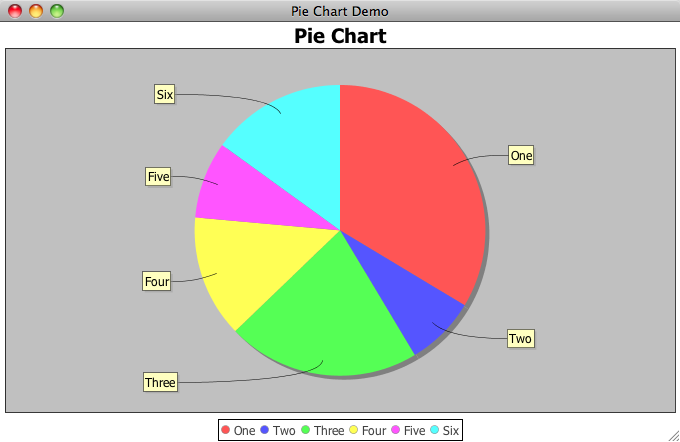
\includegraphics[width=1.0\textwidth]{images/piechart}
  \caption{Example pie chart created with the JFreeChart based
    charting DSL.\label{fig:piechartex}}
\end{figure}

\section{Other Examples Used}

This section describes some other DSLs used as examples. They have not
been written as part of the work, but are used as examples as they are
popular DSLs being used.

\subsection{Ruby on Rails}

Ruby on Rails is a framework for web development. It is implemented as
an embedded DSL in Ruby. The main Rails feature focused on in this
thesis is the \texttt{ActiveRecord} classes, providing functionality
for querying databases. The \texttt{ActiveRecord} can be seen as a
separate DSL on its own. An example of using \texttt{ActiveRecord} is
shown in listing \vref{lst:activerecordex} (from\cite{rails}). The
relationship between tables in the database is directly mapped to Ruby
classes, using a very specific syntax.

\begin{lstlisting}[float,language=ruby,caption={[Ruby on Rails \texttt{ActiveRecord} example]Example using the Ruby on Rails \texttt{ActiveRecord} database querying classes.},label=lst:activerecordex]
class Client < ActiveRecord::Base
  has_one :address
  has_one :mailing_address
  has_many :orders
  has_and_belongs_to_many :roles
end

class Address < ActiveRecord::Base
  belongs_to :client
end

class MailingAddress < Address
end

class Order < ActiveRecord::Base
  belongs_to :client, :counter_cache => true
end

class Role < ActiveRecord::Base
  has_and_belongs_to_many :clients
end
\end{lstlisting}

\subsection{Hibernate}

Hibernate is a so called object-relational-mapping (ORM) framework
written in Java. It provides much the same functionality as the
\texttt{ActiveRecord} mechanism described in the previous sections,
but implemented in Java using annotations. In listing
\vref{lst:javahibernate}, the \texttt{Client} class from the Ruby on
Rails example given in \vref{lst:activerecordex} is implemented in
Java using Hibernate.

\begin{lstlisting}[float,language=java,caption=Java Hibernate example,label=lst:javahibernate]
@Entity
public class Client

  @ManyToOne
  public Address getAddress();

  @ManyToOne
  public Address getMailingAddress();

  @OneToMany
  public List<Order> getOrders();

  @ManyToMany
  public List<Role> getRoles();
}
\end{lstlisting}

\subsection{Testing Frameworks}

Several frameworks for automated unit testing are good examples of
embedded DSLs on the JVM. In this thesis jMock\footnote{jMock -- A
  Lightweight Mock Object Library for Java:
  \url{http://www.jmock.org/}} and ScalaTest\footnote{ScalaTest --
  Open-source testing framework for Scala:
  \url{http://www.scalatest.org/}} have been used as examples. jMock
is written in Java, and is a framework providing functionality for
mocking dependencies so that classes can be tested in
isolation. ScalaTest is written in Scala, and is a unit testing
framework that facilitates several different styles of testing. Both
jMock and ScalaTest are excellent examples of frameworks taking full
advantage of their respective host languages.

\subsection{Query Languages}

Many programming languages provide APIs for general querying. A good
example is the LINQ (Language Integrated Query)\footnote{LINQ website:
  \url{http://msdn.microsoft.com/en-us/library/bb308959.aspx}} found
in the C\# language from Microsoft. LINQ has been included as an
example to provide a basis for comparison with the alternatives that
exist on the JVM.

\clearpage{\pagestyle{plain}\cleardoublepage}

\chapter{Syntax}
\label{chp:syntax}

\textit{The syntax of a language defines its surface
  form.}\cite{fri08}

It is the set of rules that define the combinations of symbols that
are considered to be correctly structured programs in that
language. For an embedded DSL its syntax describes special ways to use
the host language. Or in other words what defines the code as an
embedded DSL is the way the syntax constructs of the host language are
used, while the semantics stay the same. This chapter describes
various programming language concepts that can be useful when
designing an embedded DSL. These concepts form the building blocks
that one can choose from when building a DSL. Choice of language
determines what features will be available.

\section{Function Chaining/Nesting}
\label{sec:functionchaining}

As mentioned in section \vref{sec:embeddeddsl}, Fowler and Evans have
used the term \texttt{fluent interfaces} to describe libraries that
can be used in a certain way. A key functionality when creating such
fluent interfaces in Java is the ability to chain/nest functions
together.

One of the simplest ways to create a DSL-like syntax is to allow
chaining several function calls together. As an example consider the
following Java-code (from\cite{fow06}), where the construction of a
\texttt{HardDrive} object is shown with and without method chaining:

\begin{lstlisting}[language=java,caption=Java function chaining example.,label=lst:javafuncchain]
// Construct with setter methods
HardDrive hd = new HardDrive();
hd.setCapacity(150);
hd.setExternal(true);
hd.setSpeed(7200);

// Construct with method chaining
HardDrive hd = new HardDrive().capacity(150).external().speed(7200);
\end{lstlisting}

The chaining of methods can also be combined with method nesting,
grouping methods that belong together (also from\cite{fow06}). An
example of this is shown in listing \vref{lst:javachainnest}.

\begin{lstlisting}[float,caption=Java method chaining and nesting.,label=lst:javachainnest,language=java]
computer(
  processor(
    cores(2),
    Processor.Type.i386
  ),
  disk(
    size(150)
  ),
  disk(
    size(75),
    speed(7200),
    Disk.Interface.SATA
  )
);
\end{lstlisting}

In\cite{fre06}, this technique is described in detail. In the testing
framework \texttt{jMock} a carefully designed set of interfaces and
factory builder objects allow method chaining maintaining the wanted
order of method calls. The referred paper is a very good read
demonstrating how to design and build a library as an embedded DSL in
Java.

Function chaining is available in most programming languages. In
functional programming it is a fundamental concept, while in
object-oriented languages more a design choice (as in the example
above). In\cite{hud96}, a technique using monads in Haskell is used to
create functions that can be combined in various ways to create
embedded DSLs. Similar examples could be created in Clojure and Scala
to run on the JVM.

TODO: more about interfaces/ordering of method calls.

\section{Static Methods/Singleton Objects}

In object-oriented languages functions are nested inside classes. In
order to be able to call functions without instantiating objects we
have static methods, that are associated directly with the class
instance and not with objects created from the class. The following
example shows how to sort a list of strings in Java, using the static
method \texttt{sort} in the \texttt{Collections} class:

\begin{lstlisting}[language=java,caption=Java static sort example.,label=lst:javastaticsort]
// Create a list of strings
List<String> names = ...

// Sort the list using the static sort method in the Collections class
Collections.sort(names);
\end{lstlisting}

A different approach to static methods is the singleton objects found
in Scala. Instead of having methods defined as static there is a
notion of a singleton object, as in the following example defining
sorting similar to the Java-example above:

\begin{lstlisting}[caption=Scala singleton object sort example.,label=lst:scalasingletonsort]
// Define ListSorter object
object ListSorter {
  def sort(list: List) { ... }
}

// Use object
var names = List("name1", "name2")
ListSorter.sort(names)
\end{lstlisting}

Static methods may play a central role in an embedded DSL, especially
combined with \texttt{Member Imports} (next section). They are
typically used for object creation through patterns like
\texttt{Factory method}\footnote{The factory method is an
  object-oriented pattern that handles the creation of objects without
  specifying the exact class of the object\cite{gam95}.} and
\texttt{Builder}\footnote{The builder pattern is an object-oriented
  pattern that assists the creation of variations of objects through a
  series of abstract method calls\cite{gam95}.}, or other utility
operations like the sorting shown in the examples above. In the image
processing DSL (described in section \vref{sec:dslimageprocessing}),
singleton objects are used to construct objects. An example is shown
in listing \vref{lst:scalaimgsingleton}.

\begin{lstlisting}[float,caption=Scala image processing singleton objects.,label=lst:scalaimgsingleton]
// Using singleton object:
val squareElement = StrEl(Square, 3) // 3x3 square element
val lineElement = StrEl(HLine, 5) // 5x1 line element

// Without singleton object, using new:
val squareElement = new StrEl(Square, 3)
val lineElement = new StrEl(HLine, 5)
\end{lstlisting}

\section{Member Imports}

With member imports it is possible to make members of a class
available directly in the code that is being written. Member imports
is a very useful mechanism in object-oriented languages for creating
concise syntax, and thus in the embedding of DSLs. Java supports
importing static members of classes, both methods and constants. Using
static member import the Java sorting example from previous section
can be written as the code in listing \vref{lst:javastaticimport},
omitting the name of the \texttt{Collections} class where the
\texttt{sort} method is used.

\begin{lstlisting}[language=java,caption=Java static member import example.,label=lst:javastaticimport]
import static java.util.Collections.*; // Import all static members of the Collections class
...

// Create a list of strings
List<String> names = ...

// Sort the list
sort(names);
\end{lstlisting}

In Scala member imports are less restricted than in Java. They can be
used anywhere in the code (not just at the start of the file), and are
not restricted to static members.

\begin{lstlisting}[caption=Scala member import example.,label=lst:scalamemberimport]
class Fruit(val name: String, val color: String) // Define class Fruit with two members

val apple = new Fruit("apple", "red") // Create apple as instance of Fruit

import apple._ // Import all members from object apple

println(name + " is " + color) // Access members 'name' and 'color' directly
\end{lstlisting}

The image processing DSL uses a number of member imports to enable a
concise syntax when working with the DSL, allowing the user of the DSL
to use the method/type names directly (such as the
\texttt{loadImageFile} method and the \texttt{Square} type in the
example below):

\begin{lstlisting}[caption=Scala image processing member imports.,label=lst:scalaimgmemberimport]
import simage.io.SImageIO._
import simage.structs._
import simage.structs.StrElType._

val img = loadImageFile("cell.jpg") // Would be SImageIO.loadImageFile without member import
val se = StrEl(Square, 3) // Would be ...StrElType.Square

saveImage(img.avg(se), "cell_avg.jpg") // Would be SImageIO.saveImage without member imports
\end{lstlisting}

\section{Method Names and Operator Notation}
\label{sec:methodnames}

When constructing an embedded DSL we like to make the syntax reflect
the actual domain as much as possible. Having flexible ways to name
and call methods can be a very useful property of a host language.

Scala has two features regarding method names and syntax that are
interesting with regards to DSL development\cite{dub06}:

\begin{itemize}
\item Arbitrary method names - Scala methods can have special
  characters as names. As such Scala has full support for operator
  overloading, as operators are just regular methods with special
  names. For example \texttt{+}, \texttt{!=} and \texttt{<=}.
\item Operator notation - Methods in Scala can be called without the
  dot and parentheses.
\end{itemize}

The following example shows how the operator notation is used together
with the \texttt{+} method name in a simple matrix DSL (being an
important part of the larger image processing DSL shown in section
\vref{sec:dslimageprocessing}):

\begin{lstlisting}[caption=Scala operator notation function example.,label=lst:scalaoperator]
abstract class Matrix {
  // Method names can be operators
  def +(other: Matrix) = add(other)
  // Regular method name
  def add(other: Matrix): Matrix // Abstract method
}

// Usage example - regular notation
val m3 = m1.+(m2)
val m3 = m1.add(m2)
// Operator notation
val m3 = m1 + m2
val m3 = m1 add m2
\end{lstlisting}

Combining the method naming in Scala with method chaining can give
``fluent interfaces'' with even more concise syntax than what was
shown in previous sections. The following example is from the website
of ScalaTest, a testing framework supporting Behaviour Driven
Development\footnote{BDD is a software development technique first
  introduced in\cite{nor06}. It aims at writing automated tests in a
  natural language, and has been implemented as embedded DSLs in a
  number of different languages.} in a very fluent style:

\begin{lstlisting}[caption=Scala ScalaTest example.,label=lst:scalatest]
import org.scalatest.FlatSpec
import org.scalatest.matchers.ShouldMatchers

class StackSpec extends FlatSpec with ShouldMatchers {

  "A Stack" should "pop values in last-in-first-out order" in {
    val stack = new Stack[Int]
    stack.push(1)
    stack.push(2)
    stack.pop() should equal (2)
    stack.pop() should equal (1)
  }

  it should "throw NoSuchElementException if an empty stack is popped" in {
    val emptyStack = new Stack[String]
    evaluating { emptyStack.pop() } should produce [NoSuchElementException]
  }
}
\end{lstlisting}

In the dynamic language Ruby they have a similar mechanism to
Scala. Here you are allowed to leave the parentheses surrounding the
parameter(s) out, but not the dot in front of the method name. In
addition it is a common idiom in Ruby to append method names with a
question mark if the method returns a boolean value. Some examples of
use are shown in listing \vref{lst:rubyparam}.

\begin{lstlisting}[float,language=Ruby,caption=Ruby parameter example.,label=lst:rubyparam]
name = "John"

# Method without parameters
name.empty?()
name.empty?

# Method with one parameter
name.include?("e")
name.include? "e"
\end{lstlisting}

\section{Special Syntax Constructs}

Many programming languages have special constructs that are made
specifically to enable the writing of concise statements. Typically
constructs that only offer a different syntax that will be replaced by
the compiler at early phases of compilation. The next sub-sections
describe some examples of such mechanisms.

\subsection{The ``magic'' \texttt{apply} Method}
\label{sec:applymethod}

Scala uses the \texttt{apply} method to let classes and object define
functionality that appears to be native in the language. You can leave
the method name out and simply write syntax that seems to pass
parameters directly to an object. In the following example the
\texttt{apply} method is used to index the \texttt{Matrix} class as if
it was a native feature:

\begin{lstlisting}[caption=Scala \texttt{apply} method example.,label=lst:scalaapply]
class Matrix[T] {
  def apply(row: Int, col: Int): T = ...
}
val intMatrix = ... // Matrix[Int]
// Get Int at position 2, 4
val intVal = intMatrix(2, 4) // Replaced by compiler: intMatrix.apply(2, 4)
\end{lstlisting}

The \texttt{apply} method can also be used for object construction
without using the \texttt{new} keyword, and without exposing the
actual class being used to create the object. This makes it possible
to create code according to the factory method pattern\cite{gam95}, as
in the following example (simplified version of Matrix structure):

\begin{lstlisting}[caption=Scala \texttt{apply} method factory example.,label=lst:scalaapplyfactory]
abstract class Array2DMatrix[T](elements: Array[T]) extends Matrix[T] {
  ... // Some abstract specialization of the Matrix class
}

class IntArray2DMatrix(elements: Array[Int]) extends Array2DMatrix[Int](elements) {
  ... // Concrete implementation of an int matrix
}

// Singleton object being used to create instances of IntArray2DMatrix
object Matrix {
  def apply(ints: Int*) = new IntArray2DMatrix(Array(elements: _*))
}

// Example use, create matrix from a number of integers - hiding details about the classes shown above
val matrix = Matrix(1, 2, 3, 4, 5, 6, 7, 8)
\end{lstlisting}

As we can see from the above example, combining singleton objects with
the \texttt{apply} method can effectively hide a complex
object-oriented underlying structure. The user of the DSL can focus on
only the details that are relevant (as the list of numbers making up
the matrix in the example above, implementation details being
irrelevant).

\subsection{Query Syntax}
\label{sec:querysyntax}

In C\# 3.0 a DSL called LINQ (Language Integrated Query) was
introduced. It is used to natively query data in the language. The
implementation of the DSL relies on a number of language features
(type inference, anonymous types, object initializer and lambda
expressions -- see sections below) in addition to the query syntax
itself. An example is shown in listing \vref{lst:linq}.

\begin{lstlisting}[language={[Sharp]C},caption=C\# LINQ example.,label=lst:linq]
// Query syntax:
var results = 
  from c in SomeCollection
  let x = someValue * 2
  where c.SomeProperty < x
  select new {c.SomeProperty, c.OtherProperty};

// Resulting rewritten syntax:
var results =
  SomeCollection.Where(
    c => c.SomeProperty < (SomeValue * 2)
  ).Select( c => new {c.SomeProperty, c.OtherProperty} );
\end{lstlisting}

In Scala we have \texttt{for comprehensions} that can be viewed as a
query syntax much like that of LINQ. Complex expressions using the
mechanism will be rewritten to a combination of \texttt{filter},
\texttt{flatMap} and \texttt{map}:

\begin{lstlisting}[caption=Scala \texttt{for comprehension} example.,label=lst:scalafor]
// "Query syntax" - for comprehension:
val results = for {
  name <- listOfNames
  if (name startsWith "E")
} yield { name toUpperCase }

// Resulting rewritten syntax:
val results = listOfNames.filter(_ startsWith "E").map(_ toUpperCase)
\end{lstlisting}

Daniel Spiewak has written a paper investigating the possibility to
extend the for comprehensions in Scala to support LINQ-style database
queries\cite{spi09}. Both mechanisms rely on monadic behaviour
(concept from functional programming), where complex statements can be
constructed by combining a set of basic functions (as shown in the
examples above).

Clojure supports a mechanism that is similar to the query languages
described above, namely relational algebra on the \texttt{Set}
data-structures\cite{hal09}. As with the Scala for-comprehensions the
whole system relies on a small number of functions (set union, set
difference, rename, selection, projection and cross product), that can
be combined in various ways. Code listing \vref{lst:cljrelalg} shows a
small example of use (taken from\cite{hal09}), extracting data from
sets containing information about compositions, composers and nations.

\begin{lstlisting}[language=lisp,caption=Clojure relational algebra example.,label=lst:cljrelalg]
(project
  (join
    (select #(= (:name %) "Requiem") compositions)
    composers)
  [:country])
\end{lstlisting}

\section{Type Inference}

With type inference the compiler will figure out the type of a value
or function, so there is no need to explicitly specify it. This is
useful when writing embedded DSLs, to give a less verbose and more
concise syntax. Some examples were given in the previous section about
query syntax.

The Scala compiler will try to infer the types used. So if the type is
obvious there is no need to specify it:

\begin{lstlisting}[caption=Scala basic type inference example.,label=lst:scalabasictypeinference]
val i = 42 // Type Int is inferred
val d = i + 2.1 // Type Double is inferred
val iBy2 = (i: Int) => i * 2 // Return value Int is inferred from int parameter
val dBy2 = (i: Double) => i * 2 // Return value Double is inferred from int parameter
\end{lstlisting}

This makes the code similar to that of a dynamically typed
language. An advantage when working with embedded DSLs in dynamic
languages is that there is no need to explicitly write the types. With
Ruby or Groovy the first two definitions in the example above could
simply be written as in listing \vref{lst:rubyvariabledefs} (not even
needing the \texttt{val} used in Scala). Type errors would, however,
not be discovered until runtime. With Scala the type errors will still
be captured at compile-time, so type inference is a way to write more
concise code without loosing the safety-net provided by the compiler.

\begin{lstlisting}[language=ruby,caption=Ruby/Groovy variable definitions.,label=lst:rubyvariabledefs]
i = 42
d = i + 2.1
\end{lstlisting}

In the image processing DSL there is extensive use of the type
inference mechanism. As we can see from the example in listing
\vref{lst:scalatypeinference} there is no explicit naming of the types
involved, as opposed to the bottom part where the same code is given
with the types. As the \texttt{avg} function is specified in the
\texttt{Standard} trait being used with the \texttt{GrayScaleImage}
the full type ``GrayScaleImage with Standard'' must be given, as well
as the \texttt{Int} type parameter to the \texttt{StrEl}. The example
also displays the part type inference plays in hiding the
implementation details from the user of the DSL. With type inference
the user does not need to be aware of the types returned (what traits
are used and so forth).

\begin{lstlisting}[caption=Scala type inference example.,label=lst:scalatypeinference]
val img = loadImageFile("cell.jpg")
val se = StrEl(Square, 3)
val blurredImg = img.avg(se)

// Without using type inference the code would look like this:
val img: GrayScaleImage with Standard = loadImageFile("cell.jpg")
val se: StrEl[Int] = StrEl(Square, 3)
val blurredImg: Image = img.avg(se)
\end{lstlisting}

\section{Implicit Type Conversion}
\label{sec:implicit_type_conversion}

Implicit type conversions are used to allow the compiler to
automatically convert one type to another where possible. From a DSL
syntax perspective this is used to "add" new methods to existing
types. This can be built-in types or user-defined types. In the
following Scala example an implicit conversion is used to convert from
\texttt{Int} to \texttt{MyInt}, and thus allowing the
\texttt{doubleIt} method to be called directly on the integer value:

\begin{lstlisting}[caption=Scala implicit type conversion example.,label=lst:scalaimplicitconversion]
// Wrapper class for int
class MyInt(val i: Int) {
  def doubleIt = i * 2 // Method
}
// Implicit conversion
implicit def fromInt(i: Int) = new MyInt(i)
// Convert Int to MyInt and call method
val ten = 5.doubleIt
\end{lstlisting}

Implicit conversions are commonly used when creating embedded DSLs in
Scala. A good example is found in the ScalaTest example shown in
section \vref{sec:methodnames}, where the \texttt{String} type is used
as if it had defined the methods \texttt{should} and \texttt{in}. The
value returned from the \texttt{pop} operation on the stack being
tested is treated the same way. The relavant parts of the example is
shown in the bottom part of listing
\vref{lst:scalatestimplicitconversion}. What makes this possible is
implicit conversions, shown in the upper part of the same code
listing. For the \texttt{String} class the \texttt{should} method is
defined in a class called \texttt{StringShouldWrapper}, which is
implicitly available since there is defined a conversion from
\texttt{String}. The value popped off the stack is converted to a
\texttt{AnyShouldMatcher} with a similar implicit conversion,
including a generic type parameter.

\begin{lstlisting}[float,caption={[ScalaTest implicit conversion example]ScalaTest example using implicit type conversions.},label=lst:scalatestimplicitconversion]
// Method definitions
implicit override def convertToStringShouldWrapper(o: String): StringShouldWrapper

implicit def convertToAnyShouldWrapper[T](o: T): AnyShouldWrapper[T]

// Usage example showing relevant parts
...
"A Stack" should "pop values in last-in-first-out order" in {
...
  stack.pop() should equal (2)
  stack.pop() should equal (1)
}

it should "throw NoSuchElementException if an empty stack is popped" in {
...
\end{lstlisting}

In dynamic languages a mechanism that can give much the same results
is Monkey Patching described in
section \vref{sec:monkey_patching}. Implicit conversions are also very
useful when combining DSLs. This is described in
section \vref{sec:combining_dsls}.

\section{By-name Parameters}
\label{sec:bynameparams}

In Scala, parameters to methods can be defined as by-value or
by-name. By-value is the default, and means that the parameter is
evaluated before the method is invoked. By-name is the contrast to
by-value, and means that the evaluation of the parameter happens every
time the method implementation refers to the name.

An example where this feature is used is shown in listing
\vref{lst:scalabyname}. The method \texttt{times} in the class
\texttt{DoIntTimes} has a by-name parameter \texttt{body} of type
\texttt{Unit} (means no value, much the same as \texttt{null} in
Java). The class wraps an integer value \texttt{n}, which is used in
the \texttt{times} method to evaluate the by-name parameter n
times. In the example the class is combined with an implicit
conversion from \texttt{Int}, to provide the handy DSL syntax
\lstinline{2 times ... }.

\lstinputlisting[float,caption={[Scala by-name parameter examples]Scala example combining implicit conversion with by-name parameter.},label=lst:scalabyname]{../examples/by-name-param/ByName.scala}

\section{Lambda Expressions/Anonymous Functions}

Anonymous functions, or lambda expressions, can be used as parameters
for higher-order function\footnote{Higher-order functions are
  functions that can take other functions as input parameters or
  return a function as output value, or functions that can be stored
  in variables.}. They are useful to make concise code, and avoiding
duplication. For example in the Scala for comprehensions and the LINQ
statements shown in section \vref{sec:querysyntax}, anonymous
functions play a role in allowing filtering (if-statements).

To show how anonymous functions work consider the following
example. The goal is to filter all even numbers from a list, typically
done with the modulo operator (\%). Writing this code in Java, which
does not support anonymous functions, would result in something
similar to the example in listing \vref{lst:javaforloop} using a
\texttt{for-loop} combined with an \texttt{if-statement}.

\begin{lstlisting}[language=java,caption=Java simple for-loop/if example,label=lst:javaforloop]
List<Integer> numbers = ... // Make instance of list of integers
List<Integer> evenNumbers = new ArrayList<Integer>();

for(int number : numbers) {
  if(number % 2 == 0) evenNumbers.add(number);
}
\end{lstlisting}

In a language supporting anonymous functions, the \texttt{List} class
could have a \texttt{filter} method taking a function as parameter
which is used to decide what values should be returned in a new
list. In Scala, the example in listing \ref{lst:javaforloop} could be
implemented as follows:

\begin{lstlisting}[caption=Scala basic anonymous function example]
val numbers = ... // Make instance of list of integers
val evenNumbers = numbers.filter(_ % 2 == 0)
\end{lstlisting}

It is quite clear that anonymous functions make the code much more
to-the-point and concise. In the Scala example we could leave out both
the loop and the if statement, only focusing on the actual operation
being performed (the modulo 2 equal to 0). If several different
similar operations were to be performed, the example would be even
clearer. In Java the loop would have to be repeated several times, or
at least several if-statements would have to be included in the loop,
while in Scala (or other languages supporting anonymous functions) the
operations would occur in an ordered series of filter-statements.

In my Matrix DSL I have used higher-order functions to create
general-purpose functions to perform operations spanning a given
structuring element. The signature looks like this:

\begin{lstlisting}[caption=Scala higher-order function example]
def seOp(se: StrEl[Int], op: (Seq[T]) => T): Matrix[T]
\end{lstlisting}

It might look cryptic at first, but is really quite simple. The
first parameter is a structuring element (typically spanning a small
3x3 section of the matrix), and the second is a function converting a
sequence of values to one value. The structuring element is passed
over the matrix as a window, and the operation is run for all values
covered by the element. The yielded value is set as a new value in a
new matrix, which is the final return value of the whole function. In
the image processing DSL based on the Matrix DSL this functionality is
used to implement a number of operations, using anonymous
functions. This is shown in listing \vref{lst:scalaanonfunc}.

\begin{lstlisting}[float,caption=Scala anonymous function example.,label=lst:scalaanonfunc]
val matrix: Matrix[Int] // Internal image representation as a matrix

// Use average anonymous function to create blur effect
def blur(se: StrEl[Int]) = {
  Image(matrix.seOp(se, (seq) => seq.reduceLeft(_ + _) / seq.size))
}

// Use minimizing anonymous function to create morphological erosion effect
def erode(se: StrEl[Int]) = {
  Image(matrix.seOp(se, (seq) => seq.reduceLeft(_ min _)))
}

// Use maximizing anonymous function to create morphological dilation effect
def dilate(se: StrEl[Int]) = {
  Image(matrix.seOp(se, (seq) => seq.reduceLeft(_ max _)))
}
\end{lstlisting}

These implementations should look familiar to anyone with a knowledge
of image processing, which is the target user domain of the
DSLs. Users of the image processing DSL would never have to see the
anonymous functions, but could use the function \texttt{blur},
\texttt{erode} and \texttt{dilate} directly, as shown in listing
\vref{lst:scalaipanonfunc}.

\begin{lstlisting}[float,caption={[Scala IP anonymous functions]Scala image processing functions implemented using anonymous functions.},label=lst:scalaipanonfunc]
val image = ... // Obtain image instance
val se = StrEl(Square, 3) // Create 3x3 structuring element
val blurredImage = image.blur(se)
val erodedImage = image.erode(se)
\end{lstlisting}

Anonymous functions are also available in Ruby, Groovy and
Clojure. They are often referred to/intermixed with
closures\footnote{Closures are actually anonymous functions binding a
  variable defined in a surrounding scope, but the difference is not
  important to the usages described here (or most other places,
  really).} in Ruby and Groovy, and as lambda expressions in
Clojure. Support for anonymous functions has also been discussed for
the next version of Java\footnote{Several different proposals for
  closures/anonymous functions in Java 7 have been discussed. The main
  effort is now lead by Mark Reinhold, as stated on his blog
  (\url{http://cr.openjdk.java.net/~mr/lambda/straw-man/}), and is
  documented as ``Project Lambda'' at the OpenJDK:
  \url{http://openjdk.java.net/projects/lambda/}.}.

\section{Anonymous Types}

Anonymous types allow the construction of types without a name, based
on fields. Combined with type inference this is a central feature in
the implementation of LINQ (as described in an earlier section).

Scala also supports anonymous types. An example of using anonymous
types together with type inference:

\begin{lstlisting}[caption=Scala anonymous types example.]
val person = new { val name = "John"; val age = 26 }

println(person.name + " is " + person.age + " years old..")
\end{lstlisting}

In LINQ this is used to allow selection of fields from a database or
other data structure:

\begin{lstlisting}[language={[Sharp]C},caption=C\# LINQ example using anonymous types.]
var results = 
  ... // Some query
  select new {c.SomeProperty, c.OtherProperty};
\end{lstlisting}

In the functional world of Clojure, all data-structures are basically
anonymous types. They are defined as maps of key-value pairs. The
``person'' type shown in the Scala example above can be defined very
similarly in Clojure:

\begin{lstlisting}[language=lisp,caption=Clojure data structure example.]
(def person {:name "john" :age 25})

(println (str (person :name) " is " (person :age) " years old.."))
\end{lstlisting}

\section{Object Initializer}

Object initializers provide the ability to give values to an object
while instantiating it. In C\# this can look like the following, and
is also used to select objects of a given class instead of anonymous
types from LINQ:

\begin{lstlisting}[language={[Sharp]C},caption=C\# LINQ object initializer example.]
val results =
  ... // Some query
  select new Person { Name = c.SomeProperty, Age = c.OtherProperty }
\end{lstlisting}

Scala also supports a form for object initializers, as in the
following example:

\begin{lstlisting}[caption=Scala object initializer example]
class Person {
  var name = ""
  var age = 0
}

val person = new Person { name = "John"; age = 26 }
\end{lstlisting}

In embedded DSLs this can be useful when building query-like syntaxes
like that shown for LINQ. If the properties used to construct the
objects vary, it would mean a lot of extra code if special
constructors need to be written for every combination of
properties. Just the two properties \texttt{name} and \texttt{age}
used in the above examples would result in 4 different constructors
(none, one x 2 or both properties given).

\section{Metaprogramming}
\label{sec:metaprogramming}

Metaprogramming is the writing of programs that write or manipulate
other programs (or themselves) as their data, or that do part of the
work at compile time that would otherwise be done at runtime. In terms
of embedded DSL creation, metaprogramming can be an extremely useful
mechanism. There are quite drastic differences between the studied
programming paradigms in how they provide metaprogramming, how it is
used and what you can do with it. The next sub-sections describe some
of these differences with examples.

TODO: references on metaprogramming definitions?

\subsection{Metaprogramming in Static Languages}

Java has a wide range of mechanisms associated with metaprogramming:

\begin{itemize}
\item Annotations -- Annotations were introduced to Java with version
  5 (JDK 1.5). They are used to add metadata about a program. These
  data are not part of the program itself, and can be used both at
  compile-time/deployment-time and at runtime. Deployment-time
  annotations can be used for code generation, and can be used when
  embedding DSLs.
\item Reflection -- Reflection is a way to program with concepts such
  as \texttt{class} and \texttt{method} in Java, and as such is
  considered a form of metaprogramming. Extensive use of reflection
  can have a negative effect on the performance of a Java application.
\item Aspect Oriented Programming (AOP) -- AOP has become a popular
  mechanism in many Java frameworks the last years. It is too big of a
  concept to describe in detail here, but is worth mentioning in the
  light of metaprogramming. With AOP it is possible to alter the
  behaviour of Java-code dramatically. I have, however, not looked
  detailed at AOP here as it is not really part of the Java
  language\footnote{Aspect Oriented Programming is usually implemented
    by pre-compilation, or extensive use of dynamic proxies in
    Java. Some of the most popular AOP frameworks in Java are AspectJ
    (\url{http://www.eclipse.org/aspectj/}), JBossAOP
    (\url{http://www.jboss.org/jbossaop}) and Qi4j
    (\url{http://www.qi4j.org/}).}.
\end{itemize}

An example of an embedded DSL in Java relying heavily on annotations
is the Hibernate framework, providing an object-relational mapping
between Java domain objects and database tables. The example in
listing \vref{lst:javameta} shows Hibernate in work mapping the
classes \texttt{Person} and \texttt{Address} to database tables. A
person has one address, but many persons can live on the same
address. This relationship is mapped using annotations. With these
annotations in place, Hibernate will generate the mapping (SQL-code)
needed to extract correct data from the database.

\begin{lstlisting}[caption=Java metaprogramming with annotations.,label=lst:javameta,language=java]
@Entity
public class Person {
  @Column(name="person_name", length=100)
  public String getName() { ... }

  @ManyToOne
  public Address getAddress() { ... }
}

@Entity
public class Address {
  ...
  @OneToMany
  public List<Person> getPersons() { ... }
}

// Example of use
Address adr = ... // obtain some address object
// The getPersons() method will actually run some SQL in the background fetching correct persons
for(Person person : adr.getPersons()) { ... }
\end{lstlisting}

Scala has no special mechanism for metaprogramming beyond those
offered in Java (Scala also supports annotations and reflection), and
has not been considered in this section.

\subsection{Dynamic Metaprogramming}
\label{sec:dynamicmetaprogramming}

Dynamically typed languages are able to use metaprogramming in a more
dynamic way, to add or alter method definitions at runtime. The
dynamic typing allows referring to names of functions that don't yet
exist at compile-time, while a static language would end up with a
compiler error in the same situation. Both Groovy and Ruby have
powerful support for this kind of dynamic metaprogramming.

The example in listing \vref{lst:groovymeta} shows how the mechanism
can be used in Groovy. In this case a new method is added to the Java
\texttt{String} class\footnote{Note that the \texttt{String} class is
  final in Java, but still modifiable with dynamic metaprogramming in
  Groovy.}, and the static \texttt{random} method of the \texttt{Math}
class is changed to a not-so-random implementation useful for unit
testing or other environments where you want to have full control of
returned values.

\begin{lstlisting}[caption=Groovy metaprogramming example.,label=lst:groovymeta,language=java]
// Add a "shout" method to the Java String class
String.metaClass.shout = {
  println delegate.toUpperCase()
}
"hello".shout() // prints "HELLO"

// Handy when you want to do controlled unit testing?
Math.metaClass.static.random = {
  return 42
}
\end{lstlisting}

Ruby supports dynamic metaprogramming in a manner similar to that
shown for Groovy. A typical example of a DSL utilizing metaprogramming
in Ruby is the Rails framework and the \texttt{ActiveRecord}
class. Here metaprogramming is used to specify relationships between
the classes, with respect to database relationships. The SQL code
needed to fetch related objects will be generated as new methods. In
the example in listing \vref{lst:railsmeta} this technique is shown
for the classes \texttt{Team} and \texttt{Player}. The methods
\texttt{has\_many} and \texttt{belongs\_to} are implemented in a
manner similar to the Groovy examples above, adding methods
\texttt{team} and \texttt{players} with database extraction logic to
the classes in use. A simplified example of how the
\texttt{belongs\_to} method is implemented using dynamic
metaprogramming in Ruby is shown in listing \vref{lst:rubydynmeta},
running some SQL and creating a collection of associated object
dynamically.

\begin{lstlisting}[float,caption={[Ruby on Rails dynamic metaprogramming]Ruby on Rails example showing dynamic metaprogramming.},label=lst:railsmeta,language=Ruby]
class Team < ActiveRecord::Base
  has_many :players
end

class Player < ActiveRecord::Base
  belongs_to :team
end

# Now a player will have a 'team' method returning the team
player.team

# And a team will have a 'players' method returning a collection of players
team.players.each { |team| ... }
\end{lstlisting}

\begin{lstlisting}[float,caption={[Ruby dyn. metaprogramming example]Ruby dynamic metaprogramming example.},label=lst:rubydynmeta,language=Ruby]
class ActiveRecord
  ...
  def self.has_many(arg)
    name = arg.to_s
    send :define_method, name do
      sql = "select * from #{name} where #{self.class.name.downcase!}_id = #{self.object_id}"
      # Run sql, and return new objects based on sql result
      ...
    end
  end
  ...
end
\end{lstlisting}

This dynamic style metaprogramming is one of the biggest advantages
that dynamic languages have when it comes to designing embedded
DSLs. Using annotations or other metaprogramming techniques could be
used in Java or other static languages to generate code similar to the
one generated by the rails framework. However, the client would not
know about the methods until after compiling. So programming in this
fashion in a static language would require some intermediate step of
explicit code-generation or compiling before calling the generated
methods. I think this is an extremely big differentiator when it comes
to certain kind of DSLs and programming language paradigms. A DSL like
Rails could never have been written in a static language.

\subsection{Functional Metaprogramming}

In Clojure, the only ``pure'' functional language used in this thesis,
there is no big separation between code and data. It is a
``homoiconic'' language, meaning that Clojure code is composed of
Clojure data\cite{hal09}. As such the whole concept of metaprogramming
is really just an integrated part of the language, and not necessarily
seen as a separate concept (as in the other languages). The macro
mechanism in Clojure is the key to this.

Clojure has a programmatic macro system which allows the compiler to
be extended by user
code\footnote{\url{http://clojure.org/macros}}. This means that we can
write code that produces code, which was the definition of
metaprogramming given earlier. The Clojure macros are processed in two
steps. First the macro expands/executes, and substitutes the result
back into the program. This is called \textit{macro expansion
  time}. Then it continues with the normal \textit{compile
  time}\cite{hal09}.

The code in listing \vref{lst:cljmacro} shows a Clojure macro example
(from\cite{hal09}). The \texttt{bench} macro is a simple benchmarking
tool to time how long an expression takes to complete, returning a map
containing both the result of the expression and the time it took to
execute (in nanoseconds). The \texttt{let} expression binds the
start-time to the \texttt{start\#} name, and the results of the
expression given to the \texttt{result\#} name. The symbols \texttt{`}
and \texttt{~} are used to quote and un-quote symbols in the macro
expansion. It finishes off by returning the result together with the
computed time difference. It may not look that impressive, but it is a
powerful mechanism that will not find anything similar to in any of
the other languages. In fact, much of the Clojure library is written
as macros, even the \texttt{defmacro} definition used to define macros
is itself a macro.

\begin{lstlisting}[float,language=lisp,caption=Simple Clojure macro example.,label=lst:cljmacro]
(defmacro bench [expr]
  `(let [start# (System/nanoTime)
         result# ~expr]
     {:result result# :elapsed (- (System/nanoTime) start#)}))

; Example usage
(bench (+ 2 3))
; Output: {:result 5, :elapsed 27000}
\end{lstlisting}

Clojure also has some explicit functions to work with metadata --
\texttt{meta} and \texttt{with-meta}. Some examples of use are shown
in code listing \vref{lst:clojuremeta}.

\begin{lstlisting}[float,caption=Clojure metaprogramming example.,label=lst:clojuremeta,language=lisp]
(def my-user {:login "test" :password "secret"})
; #'user/my-user
my-user
; {:login "test", :password "secret"}
(meta my-user)
; nil
(def my-cached-user (with-meta my-user {:cached-at (java.util.Date. )}))
; #'user/my-cached-user
my-cached-user
; {:login "test", :password "secret"}
(meta my-cached-user)
; {:cached-at #<Date Sat Feb 06 20:38:28 CET 2010>}
\end{lstlisting}

\section{Open Classes/Monkey Patching}
\label{sec:monkey_patching}

A monkey patch is a way to extend or modify the runtime code of
dynamic languages without altering the original source code. In DSL
creation this can be used in much the same way as implicit
conversions, by adding new functionality to built-in or other
types. In the example in listing \vref{lst:rubymonkeypatch} code we
re-implement with open classes/monkey patching the same example shown
in section \vref{sec:implicit_type_conversion} with implicit type
conversions, giving the integer class a new method \texttt{doubleIt}.

\begin{lstlisting}[float,language=Ruby,caption={[Ruby ``monkey patching'' example]Ruby example showing ``monkey patching'' on open classes.},label=lst:rubymonkeypatch]
class Integer
  def doubleIt
    self * 2
  end
end

ten = 5.doubleIt
\end{lstlisting}

TODO: DSL example?

\section{Dynamic Dispatch -- Method Missing}

Dynamic programming languages use dynamic dispatch to determine what
code to run when a message is received. This means that errors related
to missing methods are postponed until runtime. Some languages provide
interesting ways to handle these errors, that can be utilized in DSL
creation.

In Ruby there is a notion of custom dispatch behaviour that can be
controlled by the programmer. The base class, that all other classes
extend from, has a \texttt{method\_missing} method that is called by
the dispatcher as a last resort when no other method is found to
respond to a message. The default behaviour is to throw a
\texttt{NoMethodError} (similar to what would happen in Java or other
languages), but this can be overridden by extending classes.

To see how this can be used in a DSL we can look at a simplified
version of the \texttt{ActiveRecord} class from the \texttt{Rails}
framework, as shown in listing \vref{lst:rubymethodmissing}. It maps
objects to database tables and allows dynamic querying through the DSL
syntax. In the example the method named \texttt{find\_by\_username} is
mapped to data extraction functionality through the
\texttt{method\_missing} implementation.

\begin{lstlisting}[float,language=Ruby,caption=Ruby on Rails \texttt{ActiveRecord} example.,label=lst:rubymethodmissing]
class ActiveRecord
  # ...
  def self.method_missing(method_id, *arguments)
    if match = /find_(all_by|by)_([_a-zA-Z]\w*)/.match(method_id.to_s)
      # ... extract column names from match, generate and run SQL expression + map and return results
    end
  end
end

# Define class 'Person' as extension of 'ActiveRecord'
class Person < ActiveRecord::Base
end

# Query the database for person with given user name
person = Person.find_by_username "eivindw"
\end{lstlisting}

This dynamic dispatch mechanism is another example where dynamic
languages provide unique possibilities. With a static language the
missing method would result in a compiler error, and hence not be
possible to implement.

\section{Summary}

Modern statically typed languages like Scala offer some very powerful
features for building embedded DSLs, combining concepts from
object-oriented and functional programming languages. Advanced type
systems offering type interference, implicit conversions and anonymous
types provide powerful mechanisms when constructing DSLs, removing
much of the verbosity often associated with statically typed
languages.

When comparing various classes of programming languages the biggest
difference with regards to DSL syntax seems to be that between static
and dynamic languages. Even with feature rich static programming
languages like Scala there are a series of concepts from dynamic
languages which does not have a natural counterpart in the statically
typed domain. Most notably are the powerful metaprogramming features
found in many dynamic languages and the dynamic dispatch mechanism
allowing custom handling of missing methods.

\clearpage{\pagestyle{plain}\cleardoublepage}

\chapter{Composition}
\label{chp:composition}

This chapter looks at various composition techniques used when working
with DSLs. It is divided into two main sections; the first one
describing how modular composition can be useful when constructing a
single DSL, and the second showing how to combine multiple DSLs to
create new ones.

\section{Modular DSL Composition}

With modular composition I mean structuring a program such that the
implementation is spread over several separate modules. A modular
design can be useful when creating a DSL for a number of reasons. With
a loosely coupled modular implementation the DSL can easily be
extended by implementing new modules, or customized by specifying a
subset of modules to be included. In the following subsections two
different ways to create a modular composition is shown and
discussed. First an object-oriented technique involving
mixin-composition using traits is shown, and secondly functional
composition using decorators is shown.

\subsection{Traits - Polymorphic Abilities}

Scala has support for virtual types (abstract type members) and family
polymorphism\cite{ode03}, mixin composition\cite{ode05} and
higher-order genericity\cite{moo08}. These are all powerful features
that support polymorphic embedding of DSLs\cite{hof08}. This allows
building DSLs that can have several different interpretations as
reusable components. It can also be used to effectively combine
different DSLs into new ones. The paper ``Polymorphic Embedding of
DSLs''\cite{hof08} describes this in detail with examples.

A use of traits can be to split functionality in several traits and
create classes/objects with only the methods that we need. In the
example given in listing \vref{lst:scalatraits} the \texttt{Matrix}
class does not have any methods, but instances of the class can be
mixed in with traits containing various methods. Notice how the three
instances created at the end of the example all have different methods
available, because of the way they mix in different traits.

\begin{lstlisting}[float,caption=Scala traits example.,label=lst:scalatraits]
class Matrix {} // No methods

trait AvgMtx { this: Matrix =>
  def avg(): Matrix = { ... }
}

trait MorphMtx { this: Matrix =>
  def erode(): Matrix = { ... }
  def dilate(): Matrix = { ... }
}

// Matrix with only avg() method
val m1 = new Matrix with AvgMtx
// Matrix with erode() and dilate() methods
val m2 = new Matrix with MorphMtx
// Matrix with "all" methods
val m3 = new Matrix with AvgMtx with MorphMtx
\end{lstlisting}

Mixin composition is also available in Groovy and Ruby. In Groovy
there is a general mixin meta-class function available, making it
possible to combine several classes into one. An example of using this
mechanism in Groovy is shown in listing
\vref{lst:groovymixins}. Because of the dynamic typing the
\texttt{name} variable of the \texttt{Base} class is available in the
mixin-classes, as if they were subclassing the base class. This is
different from the Scala traits example, where self-type annotation
has to be used if the traits need to access any members of the classes
they are mixed in with.

\begin{lstlisting}[float,caption=Groovy mixing composition example.,label=lst:groovymixins,language=java]
class Base {
  String name;
}

class StdOp {
  def std() {
    println("std() running.." + name);
  }
}

class ExtraOp {
  def extra() {
    println("extra() running.." + name);
  }
}

Base.class.mixin(StdOp, ExtraOp);

base = new Base(name: 'Test!');
base.std(); // Base has a std() function
base.extra(); // ..and an extra() function
\end{lstlisting}

In Ruby there is a \texttt{module} concept that provides dynamic mixin
composition functionality similar to that shown above in
Groovy. Modules are a way to logically group classes, functions or
other definitions belonging together, as an advanced form of the
packages found in Java and Scala. Modules cannot be instantiated like
classes, but can be mixed in with a new or existing class to add
functionality. Given in listing \vref{lst:rubymodules} is the same
example as was shown for Groovy above, implemented using modules in
Ruby.

\begin{lstlisting}[float,caption=Ruby mixin composition using modules.,label=lst:rubymodules,language=ruby]
class Base
  @name
  
  def initialize(name)
    @name = name
  end
end

module StdOp
  def std
    puts "std() running.." + @name
  end
end

module ExtraOp
  def extra
    puts "extra() running.." + @name
  end
end

class MyBase < Base
  include StdOp, ExtraOp
end

base = MyBase.new("Test!")
base.std() # MyBase has a std() function
base.extra() # ..and an extra() function
\end{lstlisting}

Using the modular composition techniques it is possible to extract
parts of a DSL as a new one, by only including the traits (or
mixins/modules) wanted. An optimizing compiler could also utilize this
composition to only include the parts of a DSL that are actually used,
thus optimizing the size of the bytecode produced. This would be
useful if compiling the DSL for a computer with a limited amount of
resources (memory and storage), for example a mobile or other small
device having support for running Java applications.

\subsection{Functional Composition}

Multi-method example shown in \vref{lst:cljmm}.

\begin{lstlisting}[language=lisp,caption=Clojure multi-method example,label=lst:cljmm]
(defmulti my-print class)

(defmethod my-print String [s]
  (.write *out* s))

(defmethod my-print Number [n]
  (.write *out* (.toString n)))
\end{lstlisting}

TODO: write with clojure examples

\begin{itemize}
\item Multi-methods with \texttt{defmulti} and \texttt{defmethod}.
\item Metaprogramming
\item Macro decorators
\end{itemize}

\section{Combining DSLs}
\label{sec:combining_dsls}

This section describes how to combine two DSLs into a new one, mixing
the functionality of the two original DSLs.

\subsection{Implicit Conversion}

Implicit type conversions were described in section
\vref{sec:implicit_type_conversion}, in terms of DSL syntax. In this
section we will look at how implicits can be used to combine
functionality from two different DSLs. The concept is demonstrated
with an example.

The following code shows the use of the simple DSL for
statistics. Typically some kind of data-set is created with numeric
values (in this example only integer values for simplicity). The
data-set implements the methods \texttt{average}, \texttt{minValue}
and \texttt{maxValue}. In the most basic form it can be used directly
to compute the average, minimum and maximum values of a series of
integers:

\begin{lstlisting}[caption=Scala statistics DSL basic example.]
val ds = DataSet(1, 2, 3, 4, 5, 6, 7, 8, 9)

println("Average: " + ds.average) // 5.0 (double value)
println("Minimum value: " + ds.minValue) // 1 (int value)
println("Maximum value: " + ds.maxValue) // 9 (int value)
\end{lstlisting}

As a first example of using implicit conversion to apply a DSL to new
values, we want to compute statistic values for an array of words
(strings) using the data-set DSL. In the following example an implicit
conversion from string-array to data-set is utilized to find the
average, minimum and maximum word lengths. The data-set is created
using the length of the strings as input, in the implicit function
\texttt{str2DS}. It is then possible to call data-set methods on the
string-array as if it was an instance of a data-set (which in fact it
is as the compiler implicitly converts it to one on demand). The
example is shown in listing \vref{lst:scalawordstats}.

\begin{lstlisting}[float,caption=Scala word statistics example.,label=lst:scalawordstats]
val words = Array("eivind", "test", "oslo", "bekk", "scala", "elephant", "cat")

implicit def str2DS(str: Array[String]) = {
  DataSet(str.map(_.length): _*)
}

println("Average: " + words.average) // 4.86 is the average word length
println("Minimum value: " + words.minValue) // 3 is the length of the shortest word
println("Maximum value: " + words.maxValue) // 8 is the length of the longest word
\end{lstlisting}

Finally we combine the image processing DSL with the statistics DSL
using the same technique that was shown for the string-array above. An
implicit conversion is defined converting instances of
\texttt{GrayScaleImage} (image storing only one integer value per
pixel) to a data-set, making it possible to call the statistics method
to compute the average, minimum and maximum pixel values. In a way one
could say that we have defined a new ``statistical image processing
DSL'' combining the two existing DSL, all without writing any other
code than the actual conversion. A simple example is shown below:

\begin{lstlisting}[caption={[Scala implicit conv. DSL combine example]Scala example using implicit conversion to combine DSL for statistics with DSL for image processing.}]
val img = Image(Matrix(3, List(
  9, 8, 7,
  6, 5, 6,
  7, 8, 9)))

implicit def img2DS(img: GrayScaleImage) = {
  DataSet(img.data.toArray: _*)
}

println("Average: " + img.average) // 7.22 is the average pixel value
println("Minimum value: " + img.minValue) // 5 is the smallest pixel value
println("Maximum value: " + img.maxValue) // 9 is the biggest pixel value
\end{lstlisting}

As with the string-array example shown previously we see how easy it
is to mix in the functionality of one DSL with another. One could
imagine a whole environment built from small DSLs, each describing a
specialized part of the domain. For example an environment for various
numeric analysis could be built combining DSLs for image processing,
statistics, charting etc. The image processing DSL can also be
combined with the charting DSL, to visualize properties with
images. The example in listing \vref{lst:scalaipchart} loads an image,
an uses the charting DSL to draw an area diagram of its data. An
implicit conversion creates the dataset needed for the charting DSL,
counting pixels of the various values, thus resulting in a sort of
histogram over the various gray values found in the picture. Figure
\vref{fig:iphistogram} shows two images together with their
histograms, produced with the given code. As we can see, histograms
are a useful visalization of the pixel distribution in an image. The
low contrast of the first image is clearly shown with a narrow peak in
the histogram, while the better contrast of the second image is shown
with a more evenly distributed histogram.

\begin{lstlisting}[float,caption=Scala image histogram example,label=lst:scalaipchart]
val img = loadImageCP("/numbers.png")

implicit def img2DS(img: GrayScaleImage) = {
  val dataset = new DefaultCategoryDataset
  val imgData = img.data.toList
  for(i <- img.min to img.max) {
    dataset.setValue(imgData.count(_ == i), "img", i)
  }
  dataset
}

createShowWindow(
  "Histogram Window",
  ChartFactory.createAreaChart(
    "Image Histogram", "Value", "Number", img, PlotOrientation.VERTICAL, false, true, true))
\end{lstlisting}

\begin{figure}[h]
  \subfigure[Image I]{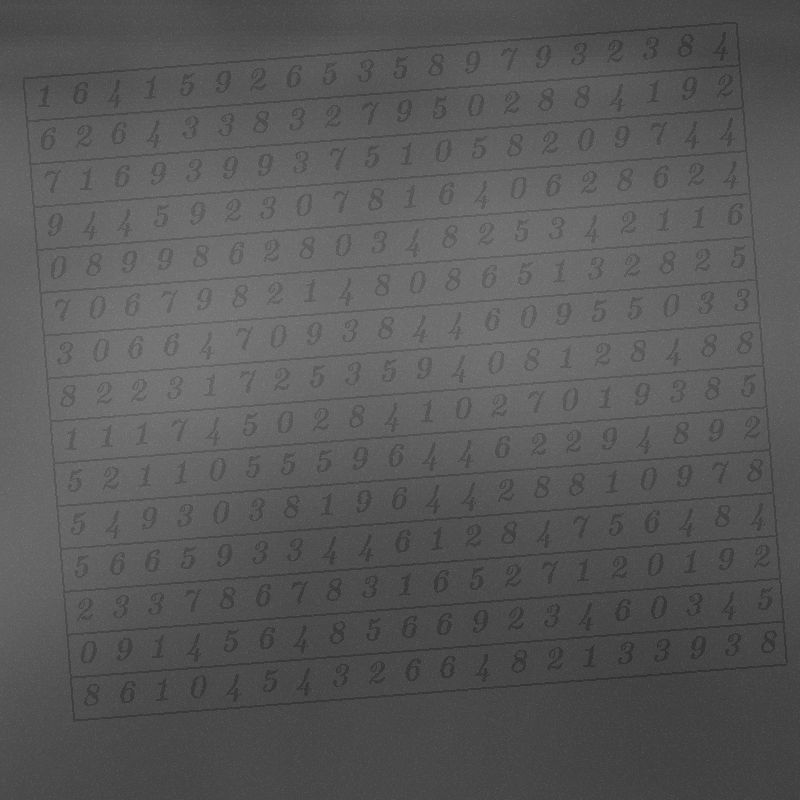
\includegraphics[width=0.49\textwidth]{images/numbers}}
  \hfill
  \subfigure[Histogram I]{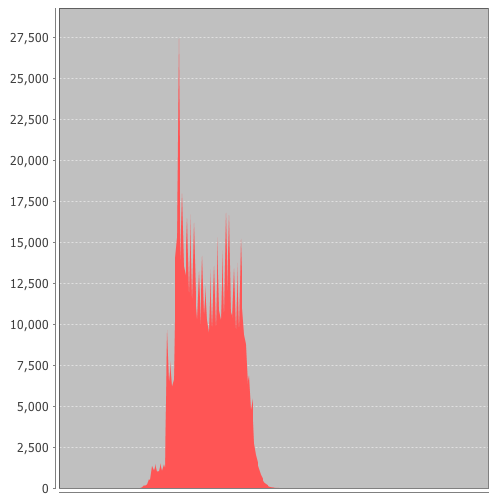
\includegraphics[width=0.49\textwidth]{images/numbers_hist}}
  \\
  \subfigure[Image II]{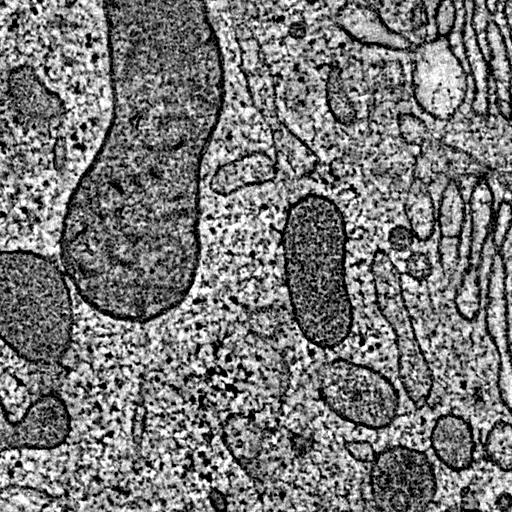
\includegraphics[width=0.49\textwidth]{images/cell}}
  \hfill
  \subfigure[Histogram II]{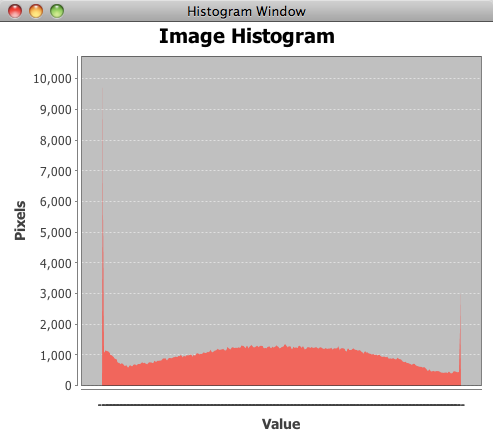
\includegraphics[width=0.49\textwidth]{images/cell_hist}}
  \caption[Two different images with generated histograms]{Two
    different images together with their generated histograms, showing
    the distribution of gray levels in the images. It clear from the
    histogram that Image II uses a much larger part of the pixel
    values available, which means it has a higher contrast, than Image
    I.\label{fig:iphistogram}}
\end{figure}

\subsection{Package Templates}
\label{sec:packagetemplates}

Package templates is an object-oriented mechanism being research by
the \textsc{swat} project at the Department of Informatics, at the
University of Oslo. Package templates extend the notion of packages in
languages like Java and Scala, with the ability to instantiate and
customize packages. The mechanism is described in detail with examples
in\cite{axe09}. This section outlines how a package template mechanism
can be utilized to combine embedded DSLs.

Having a package template mechanism in Java could be used as a sort of
multiple inheritance, as the mechanism supports merging implementation
details from several package classes into one new class. This could be
used to combine DSL classes similar to the example shown with implicit
conversions in the previous section. An example of how this could be
done is shown in listing \vref{lst:ptdsl}. Notice how the
\texttt{ImageStatistics} class constructed has methods from both the
\texttt{Image} and \texttt{DataSet} super classes, similar to what
could be achieved using traits with Scala.

\begin{lstlisting}[float,language=java,caption=Package template DSL example.,label=lst:ptdsl]
template Statistics {
  class DataSet {
    public int avg() { // Example statistical operation
      int[] data = getData();
      ... // Lots of Java code to compute and return average value
    }

    abstract int[] getData();
  }
}

template ImageProcessing {
  class Image {
    int[] imgData;

    public void blur() { ... } // Example image operation
  }
}

inst Statistics with DataSet => ImageStatistics
inst ImageProcessing with Image => ImageStatistics

class ImageStatistics with Operations {
  int[] getData() { return imgData; } // Return image data as an array
}

// Examples of use, an ImageStatistics object has both blur() and avg() methods:
ImageStatistics img = ...
img.blur();
int average = img.avg();
\end{lstlisting}

\section{Summary}

This chapter has explored ways to create modular, reusable DSL
components, as well as techniques used to combine several
DSLs. Mixin-composition, found in Groovy, Ruby and Scala, is a
powerful way to create loosely coupled modular DSLs. The functional
composition techniques in Clojure provide some exiting new ways to
compose modular code, compared to the more imperative
languages. Implicit conversion is a good technique found in Scala that
enables combining two DSLs in a very smooth manner. The package
templates mechanism research at the University of Oslo seems like a
good alternative to combine DSLs.

\clearpage{\pagestyle{plain}\cleardoublepage}

\chapter{Advanced Techniques}
\label{chp:advancedtechniques}

This chapter describes some advanced techniques that can be used in
DSL construction. More specifically it deals with operations that
remove functionality from the host language (pruning), and various
ways to extends the host language. One could discuss how relevant this
is when talking about embedding DSLs, as using these techniques widely
can alter the host languages radically. As such an embedded DSL in a
host language can be rendered to act as an external DSL, tweaking the
programming language to suit our needs.

\section{Removing from Host Language -- Pruning}

This first section deals with the removing of functionality from the
host language. It can be interesting when designing an embedded DSL to
actually deactivate constructs in the host language not being used,
and that you don't want to user of the DSL to be using either. For
instance if the DSL is written in a very functional style in the Scala
language, it might be interesting to disable some of the more
imperative mechanisms such as \texttt{while-loops}. Given this is a
pretty narrow requirement, and probably not really often needed, the
following sections just briefly discuss some of the options that
exist.

\subsection{Compiler Plugins}
\label{sec:compilerplugins}

Scala supports the notion of compiler plugins. This means that you can
write your own code that will be run as part of the compilation
process in Scala. The compiler plugin has full access to the abstract
syntax tree, and can make changes or additions as needed. The plugin
is packaged as a separate unit, and does not impact the main Scala
distribution. So if the plugin is present the functionality will be
available, but once it is removed the added functionality will not be
available anymore.

It would be quite trivial to write a compiler plugin that disables
unwanted features of Scala. For example if we wanted to remove the
\texttt{while} construct, the plugin could simply search the abstract
syntax tree for occurrences of while, and output an error message if
any are found. No examples are given here, but the Scala website
provides a good tutorial for getting started writing compiler
plugins\footnote{Writing Scala Compiler Plugins --
  \url{http://www.scala-lang.org/node/140}}.

\subsection{Pruning in Dynamic Languages}
\label{sec:dynlangprune}

Another way to prune functionality from the host language is to
utilize the open classes in Ruby, first introduced in section
\vref{sec:monkey_patching}. This can be used to redefine methods on
the base classes in the language, maybe throwing an exception or
printing an error message if an unwanted method is called. As an
example, the code in listing \vref{lst:rubyprunestring} shows an
example where the implementation of \texttt{String.length} is
redefined to print an error message.

\begin{lstlisting}[float,language=ruby,caption=Ruby String pruning example.,label=lst:rubyprunestring]
class String
  def length
    puts "Illegal method invoke!"
  end
end
\end{lstlisting}

Ruby also has some metaprogramming methods that can be used to remove
methods from base classes. The \texttt{remove\_method} method can be
used to remove a given method from the current class, while
\texttt{undef\_method} will undefine the method completely. In listing
\vref{lst:rubyundefmethod} the \texttt{String.length} is undefined
completely, rendering the message <<\texttt{NoMethodError: undefined
  method `length' for "hei":String}>> if called on the string ``hei''.

\begin{lstlisting}[float,language=ruby,caption=Ruby \texttt{undef\_method} example.,label=lst:rubyundefmethod]
class String
  undef_method: length
end
\end{lstlisting}

Similar ways to modify the base API methods and classes are also
available in Groovy, as was shown with the \texttt{random} method
redefinition in listing \vref{lst:groovymeta}.

\subsection{Pruning in Functional Languages}

Clojure has very few built-in control structures and keywords. Much of
the core functionality is defined as macros or functions in the
\texttt{clojure.core} namespace. Since Clojure is a dynamic language,
all of these macros can be redefined by the user. The code in listing
\vref{lst:cljredefcore} shows an example where the core function for
adding numbers is redefined to multiply instead. Although the example
is pretty useless, it still shows how base language functionality can
be changed. It is a powerful, but dangerous ability. Imagine the kinds
of error users would get if this was done in a number-centric DSL like
the image processing example used for this thesis.

\begin{lstlisting}[language=lisp,caption=Clojure redefining core functions.,label=lst:cljredefcore]
; Enter the clojure core namespace
(ns clojure.core)

; Redefine the add method as multiply
(def + *)

; The result of this addition will surprise the user
(+ 2 3)
\end{lstlisting}

Another way to change the core functionality of Clojure, is to use
\texttt{dynamic bindings}. With dynamic bindings it is possible to
redefine the meaning of a globally defined variable, within the scope
of a function/macro. An example is shown in listing
\vref{lst:cljbinding}\footnote{Example from
  \url{http://en.wikipedia.org/wiki/Clojure\#Examples}.}, showing how
the \texttt{noprint} macro redefines the \texttt{*out*} special
variable to a dummy \texttt{java.io.Writer} object. The \texttt{*out*}
variable is used by many functions to print information to a standard
output/console. However, because of the redefining done by the dynamic
binding, all print statements within a \texttt{noprint} macro call
will be suppressed.

\begin{lstlisting}[float,language=lisp,caption=Clojure macro binding core variable.,label=lst:cljbinding]
(def bit-bucket-writer
  (proxy [java.io.Writer] []
    (write [buf] nil)
    (close []    nil)
    (flush []    nil)))

(defmacro noprint
  "Evaluates the given expressions with all printing to *out* silenced."
  [& forms]
  `(binding [*out* bit-bucket-writer]
     ~@forms))

(println "Regular println!")
(noprint (println "Noprint println!"))
\end{lstlisting}

\section{Extending Host Language}

More interesting than removing stuff from the host language (as
discussed in the previous section) might be the ability to extend
it. If the host language does not natively support the kind of control
structure or primitive that can make your DSL as expressive as
possible, it might come in handy to be able to add that support
yourself. The following subsections describe some possibilities when
you want to extend the various host languages.

\subsection{Compiler Plugins}

The compiler plugin mechanism described in \vref{sec:compilerplugins}
may of course also be used to extend the language. Some of the new
functionality added to Scala is first introduced as compiler plugins,
and then later added to the main distribution after being tested. An
example of this is the continuations support that will be added to
Scala 2.8\footnote{A Taste of 2.8: Continuations --
  \url{http://www.scala-lang.org/node/2096}}.

\subsection{Dynamic Languages}

The mechanisms described in section \vref{sec:dynlangprune} can just
as well be used to extend the host language with new methods. Examples
of this were shown in section \vref{sec:monkey_patching}.

\subsection{Functional Languages}

Functional languages have a wide variety of ways to extend the hos
language. The first subsection below describes how functions
themselves can be written to appear as built-in keywords. The second
subsection describe Clojure macros, an extremely flexible mechanism
when it comes to extending the language.

\subsubsection{First-class Functions as Built-in Control Structures}

With functional languages it is possible to create control structures
that look like built-in keywords, but are simply first-class
functions. In Scala functions can be defined with ``pass by-name''
parameter passing, and single parameter functions can be called using
curly braces instead of parenthesis to specify the parameter (an
example was shown in section \vref{sec:bynameparams}). As an example
consider the definition of a new while construct shown in listing
\vref{lst:scalabuiltinkeywords}

\begin{lstlisting}[float,caption={[Scala built-in keyword functions]Scala example making functions look like built-in keywords.},label=lst:scalabuiltinkeywords]
def mywhile(cond: => Boolean)(body: => Unit) {
  if(cond) {
    body
    mywhile(cond)(body)
  }
}

// Example use:
var i = 0
mywhile(i < 3) {
  println("Num: " + i)
  i = i + 1
}
\end{lstlisting}

As we can see it is simple to define functions that act and look like
built-in control structures. This is very useful designing DSLs where
we want it to seem like the host language has been extended with new
features supporting the DSL.

\subsubsection{Clojure Macros}

In Clojure it is also possible to create functions as in the Scala
example in the previous section. But Clojure has a much more powerful
mechanism as well, namely the macro system. Macros in Clojure extend
the compiler by writing regular user code, and are totally different
from other programming languages macro systems. Many of the core
constructs in Clojure are in fact implemented as macros, and are not
actually primitives or other built-in support.

A macro can be seen as a kind of template that outputs code, like that
found in many other programming languages. The big difference with
macros in LISP-languages like Clojure however, is that the macro
itself is valid code and has full access to the whole language. As a
first example, consider the Clojure \texttt{unless} implementation as
a macro shown in listing \vref{lst:cljunless}.

\begin{lstlisting}[language=lisp,caption=Clojure macro adding unless,label=lst:cljunless]
(defmacro unless [expr form]
  (list 'if expr nil form))
\end{lstlisting}

To further examplify the power Clojure macros bring when it comes to
extending the host language, consider the macro in listing
\vref{lst:cljmacroreverse}. What it does is revert the order of the
statements given as arguments. The \texttt{let} statement in the
beginning defines a temporary value \texttt{rev\#} as the reverse
value of the list of arguments (\texttt{\& body}). This reversed list
is then splice-quoted back as code together with a Clojure \texttt{do}
statement. An example using the macro is shown in listing
\vref{lst:cljmacroreverseuse}. As we can see the list of statements
first provides a multiplication of two values (\texttt{x} and
\texttt{y}), then the values are defined.

\begin{lstlisting}[language=lisp,caption=Clojure macro reverting order of statements,label=lst:cljmacroreverse]
(defmacro rev [& body]
  (let [rev# (reverse body)]
    `(do ~@rev#)))
\end{lstlisting}

\begin{lstlisting}[language=lisp,caption=Clojure reverse statements example,label=lst:cljmacroreverseuse]
(def result
  (rev
    (* x y)
    (def y 4)
    (def x 3)))

(println (str "Result: " result))
; Result: 12
\end{lstlisting}

The example with the reverse macro shown above might seem pretty
useless, and it probably is. However, it was included here just to
show the amazing power released by the Clojure macro support. It would
probably prove extremely difficult to write anything like that in any
of the other languages studied in this report. Clojure gives you huge
possibilities in extending/changing the host language. The uniform and
simple syntax together with the macro system lets you build your own
language, however you want it. Just about any control structure can be
built straight into the language using macros.

\section{Summary}

There are different ways to modify the host language. With compiler
plugins, as supported by Scala, it is possible to redefine whatever
you like in the language. This does however require the use of
externally activated plugins, that must be available whenever the
functionality they provide is wanted. Dynamic languages support ways
to add methods to existing base classes, as well as removing or
redefining methods.

The most exiting capabilities in changing the host language is found
using macros in Clojure. They are an integrated part of the language,
but can still redefine existing functionality or add all kinds of new
structures. Much of the base functionality in Clojure is actually
built using macros, as opposed to being integrated as separate
keywords.

\clearpage{\pagestyle{plain}\cleardoublepage}

\chapter{Exploring Ways to Use Embedded DSLs}
\label{chp:dsluse}

So far the focus has been on the design/implementation of embedded
DSLs. This chapter discusses various ways to use embedded DSLs. There
are quite many ways to take advantage of a DSL, depending on what kind
of language it has been written in. The next sections describe some of
the usages identified, and how they are supported by the different
languages.

\section{API/Library}

The most common way to use an embedded DSL seems to be as a library
integrated in other application code. On the JVM this will typically
involve archiving compiled class files, or script + interpreter, in
one or more jar (Java Archive) files. These files will be included in
the classpath of the application that needs access to the library
API. The application programmer will then be able to import the
classes and use in the program code. An example is the JMock framework
in Java (also mentioned in section \vref{sec:functionchaining}). It
allows programmers writing unit tests to specify with an internal DSL
syntax how they want to mock dependencies to the code they are
testing. An example written in Java (DSL syntax mostly found in the
expectations declarations) is shown in listing \vref{lst:javaapi}.

\begin{lstlisting}[float,caption=Java example using jMock as an API.,label=lst:javaapi,language=java]
import junit.framework.TestCase;

import org.jmock.Mockery;
import org.jmock.Expectations;

public class PublisherTest extends TestCase {

  public void testSimplePublish() {
    Mockery context = new Mockery();
    Subscriber subscriber = context.mock(Subscriber.class);
    Publisher publisher = new Publisher();
    publisher.add(subscriber)
    String message = "message";
    context.checking(new Expectations() {{
      oneOf(subscriber).receive(message);
      allowing(subscriber).isAlive(); will(returnValue(true);
    }});
    publisher.publish(message);
    context.assertIsSatisfied();
  }
}
\end{lstlisting}

Another interesting thing when using the DSL as a library, is that the
language using the DSL not necessarily needs to be the same as the
host language the DSL was written in. If the DSL is compiled to
bytecode (\texttt{.class} files), it can be used from most of the
other languages running on the JVM. The example above could just as
well have been written in any of the languages used in this thesis,
for example in Scala as shown in listing \vref{lst:scalaapi} (looking
quite similar to the original Java example above).

\begin{lstlisting}[float,caption=Scala example using jMock as an API.,label=lst:scalaapi]
import junit.framework.TestCase

import org.jmock.{Mockery, Expectations}

class PublisherTest extends TestCase {

  def testSimplePublish {
    val context = new Mockery
    val subscriber = (context.mock(classOf[Subscriber])).asInstanceOf[Subscriber]
    val publisher = new Publisher
    publisher.add(subscriber)
    val message = "message"
    context.checking(new Expectations {
      oneOf(subscriber).receive(message)
      allowing(subscriber).isAlive; will(returnValue(true)
    })
    publisher.publish(message)
    context.assertIsSatisfied
  }
}
\end{lstlisting}

\section{Scripting}

A different approach to the use-as-a-library approach shown above is
to allow code written in the DSL to be run as a standalone
script. That is without the need to wrap it in some class or module
written in the host language. All the dynamic and interpreted
languages support this kind of usage. Scala, although it is a static
and compiled language, has a kind of interactive interpreter called
REPL (Read-Evaluate-Print Loop) that typically can be used to test
code on the fly. It can also be used to run Scala-code in a more
script-like way. The following script can be run demonstrating this
functionality, using the image processing DSL from
chapter \vref{chp:examples} as example (loading an image and saving a
blurred copy to a new file):

\begin{lstlisting}[caption=Scala scripting usage example.]
import simage.io.SImageIO._
import simage.structs._
import simage.structs.StrElType._

val img = loadImageFile("cell.jpg")
val se = StrEl(Square, 3)

val blurredImg = img.avg(se)
saveImage(blurredImg, "cell_blurred.jpg")
\end{lstlisting}

The script can then be run from the command line using the scala
interpreter (called with the \texttt{scala} command), assuming the
script is in a file named \texttt{ImageScript.scala} and that the
image processing DSL has it's classes packed in the jar
\texttt{simage.jar}:

\begin{lstlisting}[language=]
scala -classpath simage.jar ImageScript.scala
\end{lstlisting}

For users of the image processing DSL this means a great simplification
in the way it is run. They do not have to learn how to make classes,
objects and methods in Scala, as they would if they wanted to run the
DSL as a regular library in a Scala file (requiring at a minimum
creating an application object with a main method). As image analysis
experts are not necessarily computer programmers this might be a good
idea.

Similar examples can be given for other DSLs and using other host
languages supporting running code as a script.

\section{Interactive Console -- Interpreter}

Many of the programming languages studied have some sort of
interactive interpreter (like the Scala REPL mentioned in the previous
section). This can in many cases be configured to be used with a
specific library pre-loaded, which means it is possible to create a
custom version for working interactively with a DSL. Similar to the
scripting example shown above this opens possibilities to work with
the DSL without wrapping it in any host language code. But the main
advantage of using the DSL in an interactive console is the unique
ability it offers in issuing commands that are run directly.

The Scala REPL has an option to pre-load a file with commands on
start-up. Typically this can be used to include imports, implicit
definitions, type aliases or function definitions. Taking the example
from the previous section on scripting we can put all the import
statements into a file called PreDef.scala:

\begin{lstlisting}[caption={[PreDef file with IP imports]PreDef.scala file with image processing imports.}]
import simage.io.SImageIO._
import simage.structs._
import simage.structs.StrElType._
\end{lstlisting}

The interactive interpreter can then be started using the option
\texttt{-i PreDef.scala} as in the following example:

\begin{lstlisting}[language=,caption={[Scala REPL execution]Scala REPL execution with preloaded import statements.}]
scala -classpath simage.jar -i PreDef.scala

Loading Predef.scala...
import simage.io.SImageIO._
import simage.structs._
import simage.structs.StrElType._

Welcome to Scala version 2.7.7.final (Java HotSpot(TM) 64-Bit Server VM, Java 1.6.0_17).
Type in expressions to have them evaluated.
Type :help for more information.

scala> 
\end{lstlisting}

We can the issue the same commands used in the script example one by
one (notice the output for every line which is simply the interpreter
calling the \texttt{toString} method after printing the type on the
newly created object -- very useful for debugging purposes):

\begin{lstlisting}[language=,caption=Scala REPL image processing example.]
scala> val img = loadImageFile("cell.jpg")
img: simage.structs.GrayScaleImage with simage.operations.Standard with simage.operations.Morphology =
Image 512x512

scala> val se = StrEl(Square, 3)
se: simage.structs.StrEl[Int] = 
Array2D rows:3 cols:3
Array(1, 1, 1, 1, 1, 1, 1, 1, 1)

scala> val blurredImg = img.avg(se)
blurredImg: simage.structs.GrayScaleImage with simage.operations.Standard with simage.operations.Morphology =
Image 512x512

scala> saveImage(blurredImg, "cell_blurred.jpg")

scala>
\end{lstlisting}

From Scala version 2.8\footnote{To be released in the first part of
  2010, available as a first Beta version as of this writing.} the
REPL will have many improvements such as code completion (of
package/class/member names) and interactive debugging.

As mentioned in the beginning of this section all the studied
languages support interactive interpreters. Clojure has a REPL, much
like that shown for Scala. Ruby has an \texttt{irb} (Interactive
Ruby), and Groovy provides a Groovy-shell. These tools give all the
languages some advantages over using Java directly. The ability to
directly execute statements is extremely useful when you need to test a
piece of code. Most of the minor examples shown in this report where
implemented directly in the interactive interpreter environments, and
then copied out when working.

\section{Embedded Interpreter}

If we want to take the interactive interpreter in Scala a step further
it is actually possible to embed it in your own
application\footnote{\url{http://suereth.blogspot.com/2009/04/embedding-scala-interpreter.html}}
\footnote{\url{http://speaking-my-language.blogspot.com/2009/11/embedded-scala-interpreter.html}}
(see footnotes for some examples). This could be a very powerful way
to create a standalone application having a console or similar being
able to run DSL commands directly. For the image processing example
shown in chapter \vref{chp:examples} it would be possible to create
some kind of application combining such a console with an image viewer
window showing the results of the operations directly on an
image. This is similar to how \matlab{} works, a proven environment
for image analysis and other mathematical calculations.

I think this technique could be very useful for a number of cases. All
kinds of DSLs where you might want to see some immediate results of
your commands could be candidates. Examples could typically be
statistical, financial or graphical DSLs. A generic application might
even be reused for several different DSLs, thus being a powerful base
for building custom running environments for any embedded DSL written
in Scala (or any other language that compiles to regular Java
bytecode). A project using this approach is
Kojo\footnote{\url{http://www.kogics.net/sf:kojo}}, a programming
learning environment for children. They have their own Scala-based DSL
for programming in a visual environment, utilizing an embedded REPL
for writing and executing commands. Figure \vref{fig:kojoss} shows a
screen-shot of Kojo, with the embedded REPL in the bottom left window.

\begin{figure}
  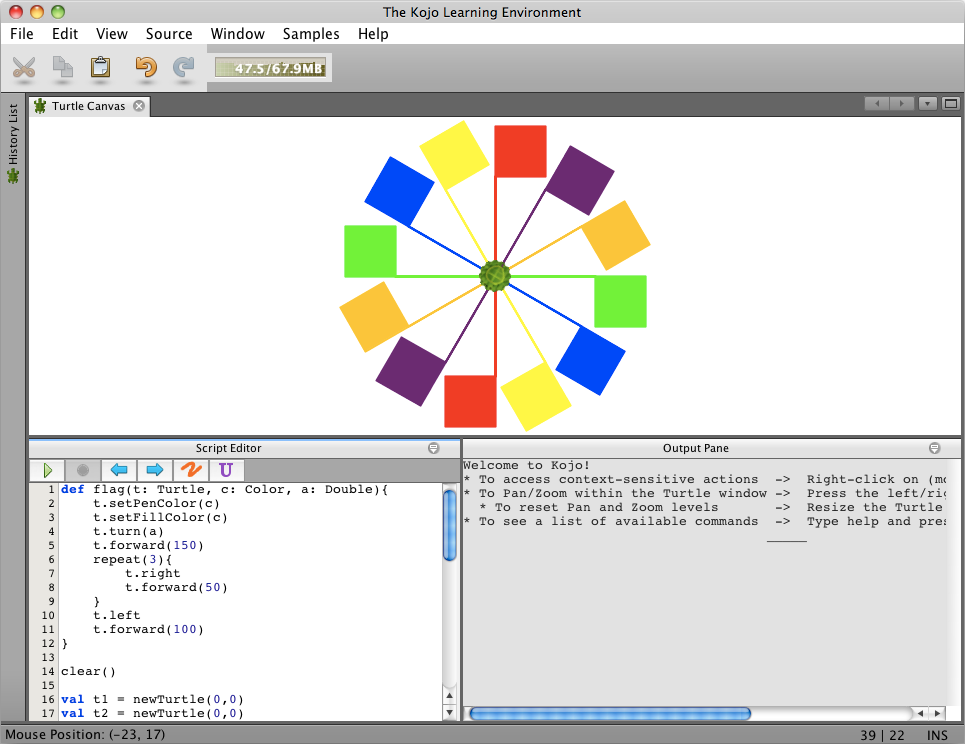
\includegraphics[width=1.0\textwidth]{images/kojo_ss}
  \caption{Screen-shot from Kojo, a programming learning environment with
    an embedded DSL-REPL.\label{fig:kojoss}}
\end{figure}

\section{Tool Support}

Since working with an embedded DSL to a large extent means dealing
with a host language, I think it is interesting to provide a brief
overview and comparison over the development tool support the various
languages offer.

\subsection{IDE -- Integrated Development Environments}

An important productivity factor when programming is having access to
a good IDE (Integrated Development Environment), helping with editing,
running, refactoring and organizing the code. Java has come a long way
in this area, with products such as Eclipse, NetBeans and IntelliJ
IDEA being central contributors to developer effectivity. Plugins
exist for all the three mentioned IDEs giving some support to all the
languages used in this thesis. For example the Image Processing DSL
was to a large extent implemented using the IntelliJ IDEA environment,
with a Scala plugin (screen-shot shown in figure
\vref{fig:intellijss}. A thorough comparison between the various
alternative environments have not been carried out, but as a general
comment it is interesting to see the difference between static and
dynamic languages. Static languages seem to be easier to implement
tools for, as much of the functionality is to some degree based on
type evaluations (for example code completion, error notifications and
refactoring).

\begin{figure}
  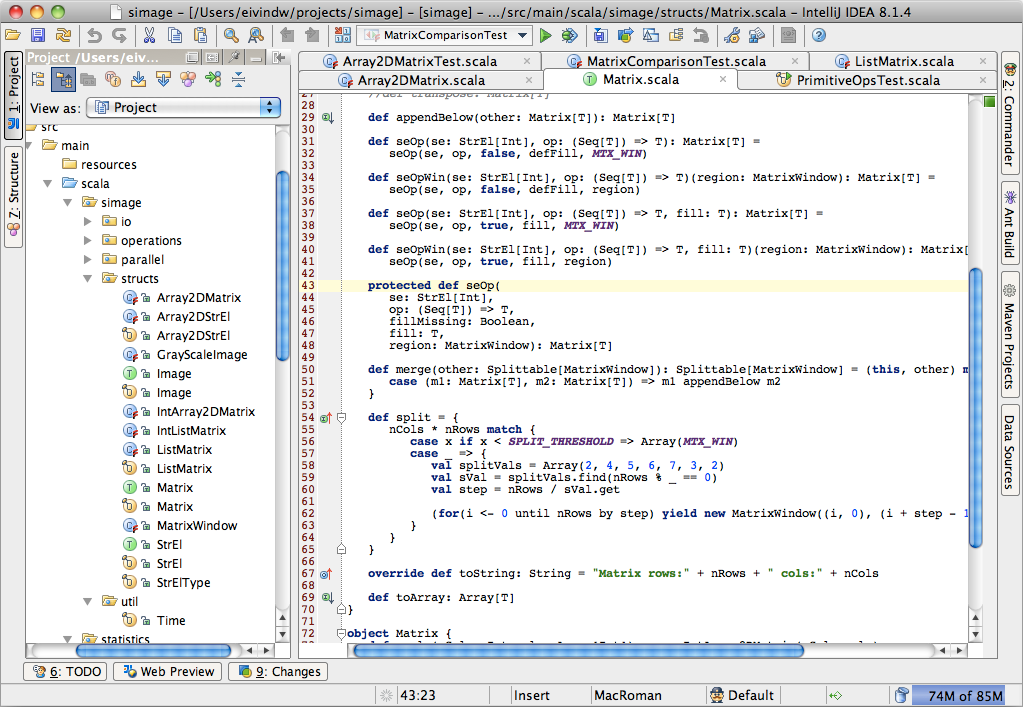
\includegraphics[width=1.0\textwidth]{images/intellij_ss}
  \caption{Screen-shot from IntelliJ IDEA, an Integrated Development
    Environment having good support for Scala.\label{fig:intellijss}}
\end{figure}

\subsection{Command Line Tools}

The Java platform has an incredible large amount of command line based
tools available, both from Sun and third party providers. Many of
these tools can be used more or less directly on all languages running
on the JVM, as they can analyze bytecode or other JVM-based management
options. Typical examples are standard Java tools like \texttt{jps},
\texttt{jstat}, \texttt{jstack} and \texttt{javap} (all included in
standard Java Development Kit
distribution\footnote{\url{http://java.sun.com/javase/6/docs/technotes/tools/}}).

Other useful tools include those that are used to automate the
building of projects (like
\texttt{make}\footnote{\url{http://www.gnu.org/software/make/}} for
unix). All the languages studied have respective alternatives, like
\texttt{rake}\footnote{\url{http://rake.rubyforge.org/}} for JRuby,
\texttt{sbt}\footnote{\url{http://code.google.com/p/simple-build-tool/}}
for Scala and
\texttt{leiningen}\footnote{\url{http://github.com/technomancy/leiningen}}
for Clojure. In addition many of the basic Java tools also work for
alternative languages. The Image Processing DSL was compiled and
tested using \texttt{Maven2}\footnote{\url{http://maven.apache.org/}},
a commonly used open source tool for building Java-projects.

\section{Error Handling}

How well does the different host languages support custom error
handling on the DSL level? Separate/different chapter? Compile-time
error handling. Dynamic versus static typing (type-safety).

\subsection{Compiler- or Runtime Errors?}

TODO: write?

\subsection{Type Errors -- Dynamic or Static Typing?}

TODO: write?

\section{Summary}

DSLs on the JVM can be used in a variety of ways; as a library,
script, directly in interpreter or even embedded with the
interpreter. All the languages studied, except Java, support some kind
of interactive interpreter/REPL. This can be used to evaluate DSL code
directly, without the need to set up a full environment with source
files.

A major advantage running a DSL on the JVM is the large amount of
tools available for the platform. Many of the tools available for the
Java language can be used directly for other languages running
bytecode on the JVM. The statically typed languages seem to have
somewhat better support for Integrated Development Environments, than
the dynamic ones.

Reporting errors, and exception handling is quite different in the
languages studied, although the basic Java exception mechanism is used
as a base for all of them. There is also a big difference between code
that is compiled first, compared to code being run on an interpreter,
when it comes to error handling. Static languages have an advantage,
in that they can discover type errors earlier than is the case with
dynamic languages. Dynamic languages seem to rely on automated unit
tests to a larger extend, to cope with the disadvantage of not knowing
the types up front.

\clearpage{\pagestyle{plain}\cleardoublepage}

\chapter{Performance}
\label{chp:performance}

This chapter looks at the performance aspects of the various DSLs and
host languages. The categories of languages are compared with regards
to performance, and some example DSLs that depend on high throughput
are implemented and analyzed. The chapter concludes with some key
points to consider when dealing with DSLs that need to run as fast as
possible on the JVM.

\section{Host Language -- Dynamic vs. Static Typing}

One of the language categorizations that potentially has a lot of
impact on the performance on the JVM is whether the language is
dynamically of statically typed. While static languages typically
perform type checking at compile-time, dynamic languages will postpone
most type checking until runtime. The JVM does, however, not support
runtime type checking very well in the current version, although some
work is being done to improve this. The next version of Java will most
likely have much better support for dynamic languages\footnote{The
  Java Community Process is developing <<JSR-292: Supporting
  Dynamically Typed Languages on the Java\texttrademark Platform>>
  (\url{http://jcp.org/aboutJava/communityprocess/edr/jsr292})},
including a specific JVM instruction (\texttt{invokedynamic}) allowing
optimizations of dynamic method invocations.

At the moment much of the dynamically typed languages on the JVM are
implemented using reflection and synthetic Java types. This makes the
code run significantly slower than that of the statically typed
languages. Some work has been done to optimize this in compiled
dynamic languages, or languages supporting some notion of just-in-time
compilation. If the type is dynamic, but still obvious to the
compiler, it is possible for the compiler to create bytecode that is
using regular static types instead. However, a thorough knowledge of
the languages and their compilers is needed to know exactly what code
will be optimized and how it should be written.

No particular benchmarks have been performed in this thesis, but
several existing ones have been studied to verify that the above
statements about dynamic languages being slower are actually
true\footnote{Several language benchmarks are published on the
  Internet, an example:
  \url{http://shootout.alioth.debian.org/}}. Most tests show that
dynamic languages are significantly slower than the static ones. The
languages studied in this thesis seem to come up in this order when
compared:

\begin{enumerate*}
\item Java -- original bytecode is the fastest.
\item Scala -- nearly as fast as Java in many cases.
\item Clojure -- uncertain about this one, but the tight coupling to
  Java suggest best performance of the three dynamic languages.
\item JRuby -- significantly slower than Java, faster than Groovy.
\item Groovy -- the slowest of all the languages studied.
\end{enumerate*}

\section{Code Efficiency}

When performing the same operation a large number of times, as is the
case with many algorithms for Image Processing, there are various
implementation related things that need to be considered. In this
section I summarize the lessons learned with regards to tuning the
code for maximum performance.

\subsection{Choice of data structures}
\label{sec:datastructures}

The underlying data structure for images and Image Processing is the
matrix. Since Scala does not include an efficient implementation of
matrix I ended up testing a few different variants:

\begin{itemize}
\item \textbf{List of Lists} -- A very logical implementation of
  matrix is by using Scala \texttt{Lists}. The idea for this
  implementation was inspired by a blog post by Jonathan
  Merritt\cite{mer08}. A simple example of using a list of lists is
  shown in figure \vref{lst:listoflist}. However, this implementation
  proves to be very slow in specific element access and iteration.
\item \textbf{2D Array} -- In Scala an \texttt{Array} will usually be
  faster than \texttt{List} because it is compiled to a native array
  in bytecode. It is also faster to implement as one flat array,
  rather than an array of arrays. This gives a much more efficient
  implementation with regards to element access and iteration. The
  implementation becomes slightly less straight-forward as we need to
  calculate the element positions in the array, as shown in figure
  \vref{lst:2darray}.
\end{itemize}

\begin{lstlisting}[float,caption={[Scala matrix list of lists]Matrix implementation based on List of Lists.},label=lst:listoflist]
class Matrix[T](val elements: List[List[T]]) {
  val nRows = elements.size
  val nCols = if(elements.isEmpty) 0
              else elements.head.size

  require(elements.forall(_.length == nCols))

  def apply(row: Int, col: Int): T = elements(row)(col)
}

val m = new Matrix(List(List(1, 2), List(3, 4)))
\end{lstlisting}

\begin{lstlisting}[float,caption={[Scala matrix 2D array]Matrix implementation based on 2D Array.},label=lst:2darray]
class Matrix[T](cols: Int, val elements: Array[T]) {
  require(elements.size % cols == 0)

  val nRows = elements.size / cols
  val nCols = cols

  def apply(row: Int, col: Int): T = elements(col + row * nCols)
}

val m = new Matrix(2, Array(1, 2, 3, 4))
\end{lstlisting}

\subsection{Iterations -- \texttt{for} comprehensions vs \texttt{while} loops}

Many Image Processing operations require some kind of calculation
performed for every element in the underlying matrix. As an example,
consider the neighbour average operation implemented using a general
structuring-element operation show in figure
\vref{lst:strelavg}. Having as efficient implementation of the
\texttt{seOp} method as possible is critical for large matrices. So
having some way of efficiently iterating over all elements of the
matrix is essential. Scala provides two basic forms of iterating;
\texttt{for comprehensions} and \texttt{while loops}:

\begin{itemize}
\item \textbf{for comprehensions} -- In Scala, for comprehensions are
  implemented as a monadic combination of the methods \texttt{filter},
  \texttt{map} and \texttt{flatMap}. This is a very powerful structure
  allowing compact and readable code. An example of implementing a
  general structuring-element operation based on for comprehensions is
  show in figure \vref{lst:forcomp}.
\item \textbf{while loops} -- For regular loops Scala provides the
  \texttt{while} keyword. Using this instead of the for comprehensions
  gives a much more iterative implementation, as shown in figure
  \vref{lst:whileloop}.
\end{itemize}

\begin{lstlisting}[float,caption={[Scala matrix neighbour average]Implementing matrix neighbour average using a general structuring-element operation.},label=lst:strelavg]
class Matrix ... {
  def seOp(se: Matrix, op: (Seq[Int]) => Int) = { ... }
}

val matrix = ... // Create matrix - load image or similar
val se = new Matrix(3, Array.make(9, 1))
val avgMatrix = matrix.seOp(se, (seq) => seq.reduceLeft(_ + _) / seq.size)
\end{lstlisting}

\begin{lstlisting}[float,caption={[Scala matrix \texttt{for-comprehension}]Implementation of a structuring element operation on a matrix using \texttt{for comprehensions}.},label=lst:forcomp]
def seOp(se: Matrix, op: (Seq[Int]) => Int) = {
  val w = se.nCols / 2
  val h = se.nRows / 2

  def seValues(row: Int, col: Int) = {
    for {
      x <- -w to w
      cx = col + x
      y <- -h to h
      ry = row + y
      if(cx >= 0 && cx < nCols && ry >= 0 && ry < nRows)
    } yield {
      elements(cx + ry * nCols)
    }
  }
  val range = for(i <- 0 until nRows; j <- 0 until nCols) yield {
    op(seValues(i, j))
  }
  new Matrix(nCols, range.toArray)
}
\end{lstlisting}

\begin{lstlisting}[float,caption={[Scala matrix \texttt{while-loops}]Implementation of a structuring element operation on a matrix using \texttt{while loops}.},label=lst:whileloop]
def seOp(se: Matrix, op: (Seq[Int]) => Int) = {
  val w = se.nCols / 2
  val h = se.nRows / 2

  val newArr = Array.make(arr.size, 0)
  var points: List[Int] = Nil
  var j, i, x, y, cx, ry = 0
  while(j < nCols) {
    i = 0
    while(i < nRows) {
      points = Nil
      x = -w
      while(x <= w) {
        cx = i + x
        y = -h
        while(y <= h) {
          ry = j + y
          if(cx >= 0 && cx < nCols && ry >= 0 && ry < nRows) {
            points = elements(cx + ry * nCols) :: points
          }
          y = y + 1
        }
        x = x + 1
      }
      newArr(i + j * nCols) = op(points)
      i = i + 1
    }
    j = j + 1
  }
  new Matrix(nCols, newArr)
}
\end{lstlisting}

\subsection{Using JVM Primitives}

In Java, there are a number of primitive types (byte, short, int,
long, float, double, char and boolean). These are not objects, but
special types with different precision. All of the primitive types
have associated wrapper types that are classes, and represented as
objects in the JVM. These wrapper classes are typically used whenever
a primitive needs to be treated as an object (for example as keys in
maps, or other collection classes). From Java 5 there is even support
for <<autoboxing>>, an implicit conversion between primitives and
their wrapper types.

However, there are performance issues related to the wrapper
classes. Using primitives is much faster than using wrappers: ``It is
not appropriate to use autoboxing and unboxing for scientific
computing, or other performance-sensitive numerical code. An Integer
is not a substitute for an int; autoboxing and unboxing blur the
distinction between primitive types and reference types, but they do
not eliminate
it.''\footnote{\url{http://java.sun.com/j2se/1.5.0/docs/guide/language/autoboxing.html}}
As stated in the quote, it is critical to ensure that primitives are
used for numerical code, like the image processing DSL in this thesis.

With languages like Scala and Clojure, there are no primitive types in
the syntax. Every value is an object (even in Clojure, being
implemented on the JVM). The Scala compiler will try to optimize where
possible, as stated in\cite{ode08}: ``The Scala compiler uses Java
arrays, primitive types, and native arithmetic where possible in the
compiled code.'' However, it is not allways obvious when this
optimization will be performed. Typically will generic collection have
some problems, even though the type parameter used is a primitive like
\texttt{Int}. Scala 2.8 will introduce some more features to help
write code that ensures the use of primitives at the bytecode
level. Most notably is the \texttt{@specialized} annotation, making
the compiler produce specialized versions of generic classes. As an
example consider the following code, defining a class \texttt{MyList}
with type parameter \texttt{T}. The compiler will produce two specific
implementations of the class, one for \texttt{Int} and one for
\texttt{Double}:

\begin{lstlisting}
class MyList[@specialized(Int, Double) T] ...
\end{lstlisting}

Clojure also has some support for specifying primitive types, dispite
the dynamic typing used throughout the language. This is called giving
the compiler ``type hints''\cite{hal09}, and can be used for
optimization. A very simple example is shown adding two integers,
first the regular Clojure way:

\begin{lstlisting}[language=lisp]
(+ 2 3)
\end{lstlisting}

The code line above would be using reflection or other similar
mechanisms used in all the dynamic languages. However, Clojure can be
used with type hints that will make the code much more efficient:

\begin{lstlisting}[language=lisp]
(+ (int 2) (int 3))
\end{lstlisting}

With code that requires maximum performance on numerical calculations
it is very important to be aware of these mechanisms. A good thing is
that one can allways write code without thinking about performance
first, and then add specializations, type hints or other mechanisms
whenever you see a need to improve the performance. Another approach
that could be done is to write the performance-critical code parts in
regular Java code, and simply include the compiled Java-classes in the
classpath of the programming language in use.

\section{Concurrency -- Parallel or Distributed Computing}
\label{sec:concurrency}

In the following sections we look at different mechanisms available
from the Scala language to achieve better performance through
utilization of the hardware resources available in the computer. The
first two sections discuss mechanisms for concurrent programming on a
multi-core/-processor environment, while the third section discuss a
mechanism for parallelization using the GPU (Graphics Processing
Unit).

\subsection{Java Concurrency}

TODO: write?

\begin{itemize}
\item Java multi-threading
\item Java futures
\item Java fork \& join in Java 7?
\end{itemize}

\subsection{Actors API}
\label{sec:actors}

The primary concurrency construct in Scala is actors. Actors are
basically concurrent processes that communicate by exchanging
messages\cite{hal06}. My first attempt at making the Image Processing
DSL parallel was by making a generic executor using the Actors
API. The result, with an example of simple usage, is shown in figure
\vref{lst:actorexecutor}. Isolated parts of the processing can be
split into separate functions that are distributed over a set of
executors. So my example with a String operation is easily extended to
Image Processing or any other domain that can be split into several
parallel functions.

The main issue with this approach is that we need to wait for the
result to be ready. This is of course not a big problem, but the next
section describes another technique that is better suited for parallel
computing.

\begin{lstlisting}[float,caption={[Scala actor executor]A generic \texttt{Executor} based on the Scala Actors API.},label=lst:actorexecutor]
import actors.Actor
import actors.Actor._

// Message contains data and transformation function
case class ExecMsg[T <: Any](data: T, op: T => T)

// Executor executes function and exits
class Executor extends Actor {
  def hasResult = result != None

  def getResult = result

  private var result: Option[Any] = None

  def act {
    while(true) {
      receive {
        case ExecMsg(d, op) => result = Some(op(d)); exit
      }
    }
  }
}

// Example usage - convert "scala" to upper case in separate thread
val exec = new Executor
exec.start // Start running - ready to receive messages
exec ! ExecMsg("scala", (s: String) => s.toUpperCase) // Send data and function
while(!exec.hasResult) {} // Busy waiting..
println("Result: " + exec.getResult.get) // Prints "SCALA"
\end{lstlisting}

\subsection{Futures API}
\label{sec:futures}

Actors may communicate using futures where requests are handled
asynchronously, but return a representation (the future) that allows
to await the reply. This is better suited for the parallel processing
we are trying to achieve. An example similar to the pure actor example
in the previous section using futures is shown in figure
\vref{lst:futureex}.

\begin{lstlisting}[float,caption={[Scala futures example]An example using \texttt{Futures} to execute a function in a separate thread.},label=lst:futureex]
import actors.Futures._

// Define function - could also be done directly in the future-block below
val func = (s: String) => s.toUpperCase

// Create future running the function with the String argument
val fut = future { func("scala" }

// Wait for and return the result
println("Result: " + fut())
\end{lstlisting}

Futures also support waiting for an array of functions to
complete. This is the mechanism used in the Image Processing DSL. See
figure \vref{lst:futureipex} for a complete example of how futures are
used to run several operation in parallel and merge the results once
all futures have finished running. The \texttt{Splittable} identifier
is simply a trait specifying \texttt{split} and \texttt{merge} methods
that need to be implemented by users of the \texttt{parallel}
function. Notice how the futures are yielded to a sequence directly
from the for comprehension and awaited completion using the
\texttt{awaitAll} function.

\begin{lstlisting}[float,caption={[Scala futures parallel mechanism]A general parallel mechanism based on futures.},label=lst:futureipex]
import actors.Futures._

object Operations {

  def parallel[T](obj: Splittable[T], op: (T) => Splittable[T]): Splittable[T] = {
    obj.split match {
      case Array(region) => op(region)
      case regions: Array[T] => {
        val futures = for(region <- regions) yield future {
          op(region)
        }
        val results = awaitAll(5000, futures: _*)
        val parts = for(result <- results) yield result.get.asInstanceOf[Splittable[T]]
        parts.reduceLeft(_ merge _)
      }
    }
  }
}

// Example usage - double values in the list in separate threads
case class MyList(val list: List[Int]) extends Splittable[Int] {
  def split = list.toArray
  
  def merge(other: Splittable[Int]): Splittable[Int] = (this, other) match {
    case (t: MyList, o: MyList) => new MyList(t.list ::: o.list)
  }
}

val splitList = MyList(List(2, 5, 7, 1))

val doubledList = parallel (
  splitList,
  (i: Int) => {
    Thread.sleep(100) // Slow things down a little
    new MyList(List(i * 2))
  }
).asInstanceOf[MyList]
\end{lstlisting}

\subsection{Functional Concurrency with Clojure}

An important factor in all functional programming is the strict
separation between mutable and immutable data structures. Where Scala,
being a multi-paradigm language, offers mutable variables and
encapsulation of state as all object-oriented languages (in addition
to offering immutable alternatives), Clojure tries to be more pure on
the functional side and hence makes immutable programming the
``default'' model in the language. All handling of state must be done
in an explicit manner, forcing the user of the language to deal with
all changes to the mutable state of a program. A program that has no
shared mutable state can easily take advantage of concurrent
programming. If you know that the same state can not be overridden by
multiple threads there is no need for explicit locking or other
mechanisms synchronizing access to the data. This is one of the major
benefits when working with functional programming languages. This
section shows how mechanisms for concurrency can be utilized in
Clojure, with some simple examples.

One of the ways Clojure integrated with Java is in making all
functions implement the \texttt{java.lang.Runnable} and
\texttt{java.util.concurrent.Callable} interfaces, from the concurrent
classes added to the JDK from version 1.5. This allows all Clojure
functions being able to run directly in separate Java threads, or
using executors or other mechanisms from the Java concurrent API. So
spawning several threads to perform separate tasks is extremely
easy. An example is shown in the following listing, where the function
printing ``hello!''  is run in a separate thread (also created
directly) on the JVM:

\begin{lstlisting}[language=lisp]
(.start (Thread. (fn [] (print "hello!"))))
\end{lstlisting}

It gets a bit more complicated when several threads need to cooperate
to solve a task, as in the Scala image processing examples shown in
previous sections. Clojure provides some different mechanisms when
working with shared data:

\begin{itemize*}
\item \textbf{Atoms} -- Single unit data that can be read/changed in
  atomic, synchronous operations.
\item \textbf{Refs} -- Shared data units that must be modified in
  Software Transactional Memory (STM), a Clojure transaction
  mechanism. Several refs can be changed in one atomic synchronous
  operation.
\item \textbf{Agents} -- Shared data units supporting asynchronous
  updates running functions on separate threads, using messages. This
  is similar to the Scala actor mechanism described in section
  \vref{sec:actors}.
\end{itemize*}

All of these mechanisms make it possible to program in a functional
way, and apply the proper concurrency terms when needing to share
state with other functions.

Another way to make Clojure code run faster is to use memoization of
functions. With memoization the result of the function is cached in
memory with the parameters as keys. Whenever a function is called with
the same parameters as before the cached result is returned
directly. So in using memoization on computationally heavy functions
we are trading CPU for memory. Less CPU will be used, as the
calculations only run once, but more memory will be consumed in
caching all the function results. A simple example, inspired from an
example in\cite{hal09}, of memoization is shown in code listing
\vref{lst:cljmemoization}. Running the example clearly shows that the
memoized version runs roughly 3 times faster as it is actually only
run two times for the given values:

\begin{lstlisting}[language=]
\$ clj-orig memo.clj 
(slow-double) "Elapsed time: 602.931 msecs"
(mem-double) "Elapsed time: 200.744 msecs"
\end{lstlisting}

\begin{lstlisting}[float,language=lisp,caption=Clojure memoization example,label=lst:cljmemoization]
; Slow function
(defn slow-double [n]
  (Thread/sleep 100)
  (* n 2))
; Memoized version of slow function
(def mem-double (memoize slow-double))

; Timing the two functions over a vector of values
(def values [1 2 1 2 1 2])
(time (dorun (map slow-double values)))
(time (dorun (map mem-double values)))
\end{lstlisting}

The memoization mechanism in Clojure would be very useful when
implementing an image processing DSL or similar requiring heavy
computations. Large parts of many images are similar, and would most
likely lead to the functions being called with the same parameters
several times when passing over the image. A memoized version would
simply return the already calculated value the second time around.

\section{Secondary Processors -- GPU}

Recent years manufacturers of graphics cards and GPUs (Graphics
Processing Unit) have made libraries available to run general code
(not just graphics processing) on their hardware. This is typically
hardware optimized for matrices and image processing, so it should be
very interesting to utilize this possibility to speed up the
operations in a Image Processing library.

OpenCL\texttrademark\cite{opencl} is an open standard for parallel
programming that utilizes the power of the GPU to perform
calculations. OpenCL is being created by the Khronos Group with the
participation of many industry-leading companies and institutions. A
Scala API exists which enables Scala programs to make use of the
possibilities offered by OpenCL -- ScalaCL\cite{scalacl}.

A simple example using ScalaCL to add two arrays of integers is shown
in figure \vref{lst:scalacl}.

\begin{lstlisting}[float,caption=Add two arrays of integers using ScalaCL.,label=lst:scalacl]
import scalacl.{Dim, Program}
import scalacl.ScalaCL._

class SeOpOCL(i: Dim) extends Program(i) {
  val iarr = IntsVar
  val iarr2 = IntsVar
  
  var output = IntsVar
  
  content = output := iarr + iarr2
}

val arr1 = Array(1, 2, 3, 4, 5)
val arr2 = Array(5, 4, 3, 2, 1)

val prog = new SeOpOCL(new Dim(arr1.size))

prog.iarr.write(arr1)
prog.iarr2.write(arr2)

prog !

println("First: " + prog.output.get(0)) // Print 6
\end{lstlisting}

\section{JVM Tuning -- JVM Arguments}

The JVM supports a wide variety of tuning/configuration options that
must be considered when optimizing an application for
performance. This section briefly describes some of these options,
with a focus on the various programming languages running on the
JVM. Configuring the JVM for performance is covered in details by
documentation provided by
Sun\footnote{\url{http://java.sun.com/javase/technologies/performance.jsp}}
\footnote{\url{http://java.sun.com/performance/reference/whitepapers/tuning.html}}.

\subsection{Configuring Memory Usage and the Garbage Collectors}

The way memory is used and reused can be configured in a wide variety
of ways on the JVM. This is common for all kinds of programs running
on the virtual machine, regardless of language implementation. It is
possible to control both the heap (where objects are stored) and stack
(where active executions are stored) sizes, setting initial values and
controlling how fast they can grow in size and the upper limits. Since
the JVM provides automatic garbage collection, setting memory limits
directly control how often the garbage collector will run. Parameters
are also available to control how the garbage collectors
run\footnote{\url{http://java.sun.com/docs/hotspot/gc5.0/gc_tuning_5.html}}.

\subsection{Configuring for Specific Programming Languages}

TODO: write.

\section{Summary}

The performance part is one of the areas where there is a big
difference between the various language categories. Dynamic languages
are significantly slower than static ones running on the JVM, due to
synthetic types and use of reflection-based mechanisms. This might
change is future releases of Java as more native support for dynamic
invocation is added to the JVM.

Functional language provide an exciting new view on concurrency, with
a focus on immutable data structures. Scala combines
object-orientation with functional programming style to enable
concurrency through a variety of mechanisms, such as actors and
futures. Clojure provides a more pure functional view, enabling
mechanisms like concurrent agents and function memoization to improve
performance.

New frameworks are appearing allowing the use of GPUs or other
secondary processors found on modern computers, potentially bringing
the performance of JVM based programs to new heights.

Several ways to tune the JVM for performance exist. These could be
used for most languages running on the JVM, although a more detailed
understanding of each language should be made to utilize this in a
best possible way.

\clearpage{\pagestyle{plain}\cleardoublepage}

\chapter{Summary}
\label{chp:summary}

This chapter first provides a conclusion of the results
found. Secondly follows a section providing a critical discussion of
the work performed. A separate section is devoted to showing
particular research contributions, that are believed to be new ideas
created during the thesis work. At last a section suggesting future
work is given.

\section{Conclusion}

This section concludes the results found during the work of the
thesis. It is divided into subsection grouping related results.

\subsection{Language Categories and Embedded DSLs}

There is no doubt that all the languages studied in this thesis work
provide much features that are not found in the Java language. This
section tries to summarize when (for what kind of tasks) the different
languages would be a good match.

The dynamic object-oriented languages (Groovy and Ruby) offer a very
concise coding-style, a central requirement when developing embedded
DSLs. Code looks very clean without information about types
included. Another extremely powerful mechanism only available in the
dynamic languages is the dynamic metaprogramming described in section
\vref{sec:dynamicmetaprogramming}. Code that dynamically generates new
code provides a basis for popular DSL environments like the Ruby on
Rails framework.

The multi-paradigm language Scala, combining object-orientation with
functional programming, offer a huge set of new capabilities when it
comes to embedded DSL design (compared to the Java language). Features
like implicit conversions, type inference and operator notation on
regular methods are just some examples. Being statically typed and
compiled still makes the language similar in many ways to Java, and
might be one of the easiest languages to learn for a Java
programmer. Scala offers, in most cases, code that is just as concise
as that of the dynamic languages, with the added benefit of being
compiled and thus checked for many errors earlier than the interpreted
languages.

The purely functional language of Clojure is maybe the most
``different'' from the rest of the languages, especially with regards
to the syntax. With the inheritance from LISP it has very few keywords
and built-in control structures. However, it sports a macro-mechanism
that is capable of creating most control structures. As such the
language is maybe one of the best suited for writing narrow and
specific DSLs, as it can be adjusted to exactly the way you want
it. The language was included in the project as an ``outsider'', but
proved its worth very quickly.

\subsection{Usage}

While a DSL written in Java will have to be compiled and used like an
API or library in other Java code, all the languages studied have
other capabilities with regards to usage.

Interpreted languages can be run directly as scripts on a JVM, and the
compiled ones include REPL-environments giving them the same
capabilities. Creating and running a script-file is significantly
faster than wrapping the functionality up in a class with a main
method, as you would have to do in Java.

The interpreters/REPL-environments can also be used directly, to run
code on the fly. This is an amazing capability when it comes to
testing code out during implementation. Another exciting use is the
ability to embed these environments directly in an application,
providing an interactive environment for the DSL directly. This would
be highly relevant for a numerical computation environment including
the example DSLs of image processing, statistics and charting.

An advantage all the languages share is the ability to utilize the
existing tools and frameworks on the JVM. Java is an extremely popular
language, and there are thousands of useful open source or other
easily available tools to choose from.

\subsection{Performance}

The biggest difference in performance between the language types is
that between dynamic and static languages. Dynamic languages running
on the JVM are significantly slower, because of synthetic types. This
might change in future versions of the JVM, as the
\texttt{invokedynamic} instruction is added to the JVM. But at the
moment a DSL that needs effective code, like those adding thousands of
numbers or similar, should probably be implemented in static languages
(like Java or Scala).

The functional languages provide ways to create very concise
code. However, some of these features seem to cost quite a lot when it
comes to performance. Some examples include for-comprehensions and
pattern matching in Scala, that are much slower than while-loops or
general if-else statements. So there is a trade-off between concise
code and high performance. Scala 2.8 might improve this a little, with
better support for JVM primitives and annotations to create effective
recursions and pattern matching statements.

The functional languages of Scala and Clojure offer very good
mechanisms for concurrency. The immutable world of functional
programming makes it very easy to create threads that cooperate in
solving problems. The biggest advantage is that they make concurrency
easy to implement without risks for deadlocks and other common
problems when working with Java concurrency.

\section{Evaluation and Discussion}

This section is meant to provide a critical self-evaluation and
discussion of the work performed. As this project is coming to an end,
I realize that there are a few things that could have been done and/or
prioritized differently.

A first observation that should be made is regarding the scope of the
project, and the programming languages included. When I started
working on this thesis I had a very good understanding and experience
with the Java programming language. All the other programming
languages were relatively new to me. The amount of time and
mindset-shifting needed to learn 3-4 new programming languages in less
than a year was seriously under-estimated. As such, a more narrow
focus with only one alternative language might have been more
effective with regards to the domain-specific language angle. For me
personally it has been an extremely interesting year, with a massive
amount of useful knowledge added, but I have a feeling that the
research contribution of the thesis could have been bigger with a
slightly more narrow focus.

Secondly one could also question the domain-specific language
focus. As it turned out, this work is much more focused on general
capabilities in different programming languages than it is focused on
domain-specific languages. Although these things are closely related,
as language features certainly are important when implementing
domain-specific languages. Maybe a more pure focus on programming
language comparison would have been better?

All in all I am still quite happy with the results of this thesis
work. I have learned many new programming languages, and certainly
gained a new understanding of what it means to work in a
research-oriented setting. As shown in section \vref{sec:futurework},
I feel that this thesis could be used as a basis for several new
master-assignments, all narrowing down on parts that the wide scope
did not allow detailing further in this report.

\section{Research Contributions}

This section summarizes research contributions made in the thesis
work. As much of the results are not new in terms of research, and
also are scattered throughout the report, it is important to gather
all the key findings in one place. The following subsections each
describe a perceived research contribution made by this thesis work.

\subsection{Package Templates for Embedded DSL Composition}

As described in section \vref{sec:packagetemplates}, package templates
is a newly researched mechanism suggesting an exiting new way to
compose Java-programs. Using this mechanism in a domain-specific
language setting is an interesting idea.

\subsection{Dynamic Features in Statically Typed Languages}

Dynamic languages have advantages with regards to metaprogramming, as
members and types can be invoked without actually existing at
compile-time. Adding some kind of dynamic support to an advanced
static language like Scala would be a very interesting experiment.

\subsection{Embedding High-Performance DSLs on the JVM}

The whole performance section, with a focus on high-performance DSL
code running in a JVM, provides a new view. Much of the JVM-DSL
related research material that has been written is entirely focused
around syntax-capabilities. The performance focus is also important
and is one of the areas suggested for further research in the sections
to follow.

\subsection{Basic Elements of Image Processing DSL in Scala}

The general idea of using Scala to build an image processing DSL also
seems like an area where there is not much research existing from
before.

\section{Suggestions for Future Work}
\label{sec:futurework}

As this thesis has a quite general of wide-spread focus, there are
several areas that could be worth researching further and in more
details. This section is divided into subsections, each describing a
separate area that deserves more attention. I believe several new
master thesis can be written from each of the suggested areas
below. The topics have been identified from working with embedded
DSLs, but are presented as more general features.

\subsection{Implementing Package Templates in Scala}

The package template mechanism described in\cite{axe09} by the
\textsc{swat} project is an advanced object-oriented mechanism that
could be implemented in Scala. Writing compiler plugins is an
available and well documented feature (discussed in section
\vref{sec:compilerplugins}) that could be utilized in this work.

\subsection{Add Support for a Dynamic Type in a Statically Typed Language}

The C\# language from Microsoft is a statically typed language that
from version 4.0\footnote{To be released spring 2010.} adds support
for a \texttt{dynamic} keyword allowing type checking to be postponed
until runtime\footnote{C\# 4.0 -- Using Type dynamic:
  \url{http://msdn.microsoft.com/en-us/library/dd264736\%28VS.100\%29.aspx}}. Features
such as this bridges much of the gap between statically and
dynamically typed languages. A suggestion of future work is to add
similar support to one of the statically typed languages running on
the JVM (as Scala or Java used in this thesis).

\subsection{Implement More Powerful Meta Programming Features in Scala}

As described in section \vref{sec:dynamicmetaprogramming} one of the
major benefits of using a dynamically typed language is the powerful
metaprogramming mechanisms. It would certainly be interesting to
research further the possibilities of adding similar support to Scala
or another statically typed language on the JVM. This task could be
done in parallel with the dynamic type support described in the
previous section.

\subsection{Create Image Processing DSL in Clojure}

Clojure is a very interesting language providing a more pure
functional programming model than Scala on the JVM. It would be
interesting investigating further using the functional capabilities of
Clojure in implementing an image processing DSL similar to the one
implemented in Scala in this thesis.

\subsection{Implement a Complete Environment for Computationally Intensive Tasks}

The main example in this thesis work has been the DSLs for image
processing, statistics and charts. Joint together these form a very
basic foundation for an environment providing a friendly syntax in
programming computationally intensive tasks.

It would be very interesting working further with these ideas,
focusing more on the specific domain of image processing and other
tasks requiring high performance computations. A JVM based environment
could potentially support several different host languages, each being
leveraged for its benefits. For example using Scala and Clojure for
concurrency, and Groovy for more dynamic queries (charting, reporting
or similar). The building blocks requiring full control of the
generated byte-code could be implemented in Java (for optimal
performance), using the other languages to provide DSL syntax and
other enhancements (like concurrency, querying, interactive
interpreter consoles ++) on top.

\clearpage{\pagestyle{plain}\cleardoublepage}

\begin{spacing}{0}
\addcontentsline{toc}{chapter}{Bibliography}
\bibliography{master}
\bibliographystyle{plain}
\end{spacing}

\end{document}

% LocalWords:  lst linq TODO boxcolor matnat textcolor programminglanguages fn
% LocalWords:  dsls plmatrix HelloWorld args println rubyhello rubyjava defn se
% LocalWords:  setDefaultCloseOperation setVisible fibonacci clojurejava javac
% LocalWords:  getProperty toUpperCase clojure getName scalajava scalacompile
% LocalWords:  javacompile jvm scalalib eximg exavg img imread jpg imgAvg StrEl
% LocalWords:  medfilt imwrite scalaimgproc loadImageCP saveImage SImageIO num
% LocalWords:  StrElType applymethod DStrEl GrayScaleImage ie chp DataSet ints
% LocalWords:  minValue maxValue statsdsl intArr reduceLeft chartdsl piechartex
% LocalWords:  createPieChart pieData activerecordex MailingAddress embeddeddsl
% LocalWords:  HardDrive hd setCapacity setExternal setSpeed javachainnest eq
% LocalWords:  jmock testAcceptsOfferIfLowPrice returnValue ListSorter HLine IP
% LocalWords:  dslimageprocessing squareElement lineElement loadImageFile BDD
% LocalWords:  StackSpec FlatSpec ShouldMatchers NoSuchElementException intVal
% LocalWords:  emptyStack intMatrix DMatrix IntArray SomeCollection someValue
% LocalWords:  SomeProperty OtherProperty flatMap listOfNames startsWith iBy Qi
% LocalWords:  dBy scalatypeinference blurredImg MyInt doubleIt fromInt seOp zA
% LocalWords:  methodnames scalatestimplicitconversion StringShouldWrapper adr
% LocalWords:  AnyShouldMatcher scalatestimplicitconversiondef AnyShouldWrapper
% LocalWords:  convertToStringShouldWrapper convertToAnyShouldWrapper ArrayList
% LocalWords:  querysyntax evenNumbers scalaanonfunc blurredImage erodedImage
% LocalWords:  javameta ManyToOne getAddress OneToMany getPersons groovymeta ds
% LocalWords:  railsmeta rubydynmeta dyn arg sql clojuremeta login CET username
% LocalWords:  NoMethodError eivindw scalatraits AvgMtx MorphMtx groovymixins
% LocalWords:  StdOp ExtraOp rubymodules MyBase cljmm defmulti defmethod str VM
% LocalWords:  toString scalawordstats conv ptdsl ImageStatistics getData undef
% LocalWords:  ImageProcessing imgData scalabuiltinkeywords mywhile cond expr
% LocalWords:  cljunless defmacro functionchaining javaapi PublisherTest oneOf
% LocalWords:  TestCase testSimplePublish isAlive assertIsSatisfied scalaapi cx
% LocalWords:  ImageScript simage PreDef Predef HotSpot clj irb groovysh JLine
% LocalWords:  IntelliJ NetBeans Refactoring listoflist darray nRows nCols ry
% LocalWords:  isEmpty forall strelavg forcomp whileloop avgMatrix seValues mem
% LocalWords:  toArray newArr actorexecutor ExecMsg hasResult getResult func ns
% LocalWords:  futureex futureipex awaitAll MyList splitList doubledList msecs
% LocalWords:  asInstanceOf cljmemoization dorun scalacl SeOpOCL iarr IntsVar
% LocalWords:  prog compilerplugins aspx dynamicmetaprogramming rubyprunestring
% LocalWords:  rubyundefmethod hei cljredefcore cljbinding noprint buf cljjava
% LocalWords:  dynlangprune invokedynamic linewidth scalastatsdsluse Kojo IDE
% LocalWords:  kojoss refactoring effectivity IDEs intellijss jps jstat jstack
% LocalWords:  javap unix sbt leiningen futurework packagetemplates
